\section{Results}

As the complete stucture to analize was symmetrical, only a half of it was modeled with a transfinite mesh and studied, as shown bellow.

\begin{figure}[H]
    \centering
    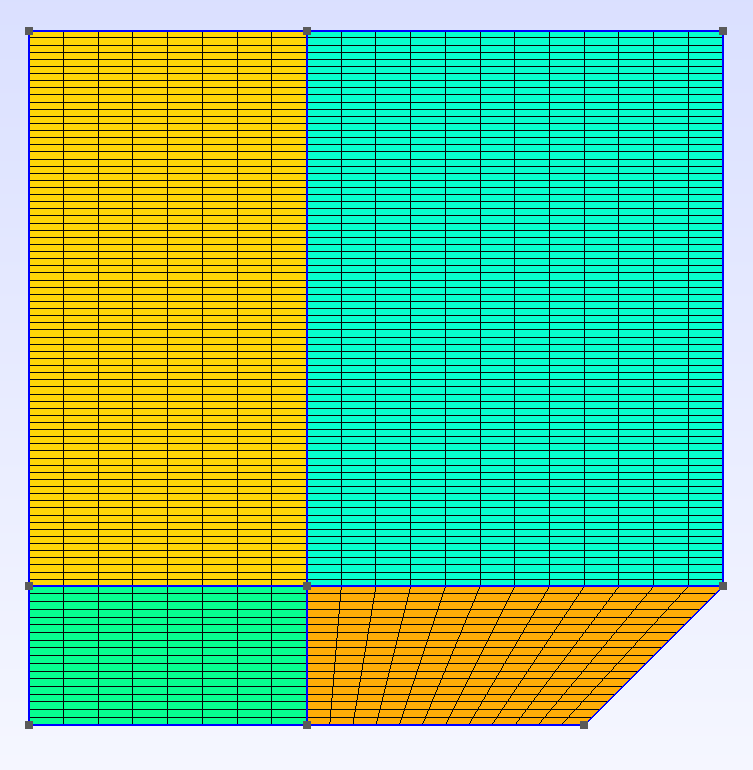
\includegraphics[width=0.5\textwidth]{img/geometria.png}
    \caption{Half structure modeled in GMSH}
    \label{fig:half_structure}
\end{figure}

\subsection{Part b) PONER LOS GRAFICOS LOCALES}

In this section, a stress analysis was made over 4 different mesh sizes using two refinment techniques, global and local refinment, for both element types.

For the global refinment, the characteristic size h was modified uniformly across the entire mesh, varying its value from 2 mm up to 1.25 mm. These values were determined based on the time required for the simulation to run and the capacity of the software to refine the mesh.

In the case of local refinment, the characteristic size h was modified in a specific region of the mesh, near the stress concentration area, in other words, the right border. For this to be studied, the number of elements was higher in that zone compared to the left border.

The results of refining the mesh globally and locally are shown in the following sections.

\subsubsection{Quad4 Element}

The following maps shows how the stress distribution changes with the mesh size as it is refined using Quad4 elements.

\begin{figure}[H]
  \centering
  \begin{subfigure}[b]{0.45\textwidth}
    \centering
    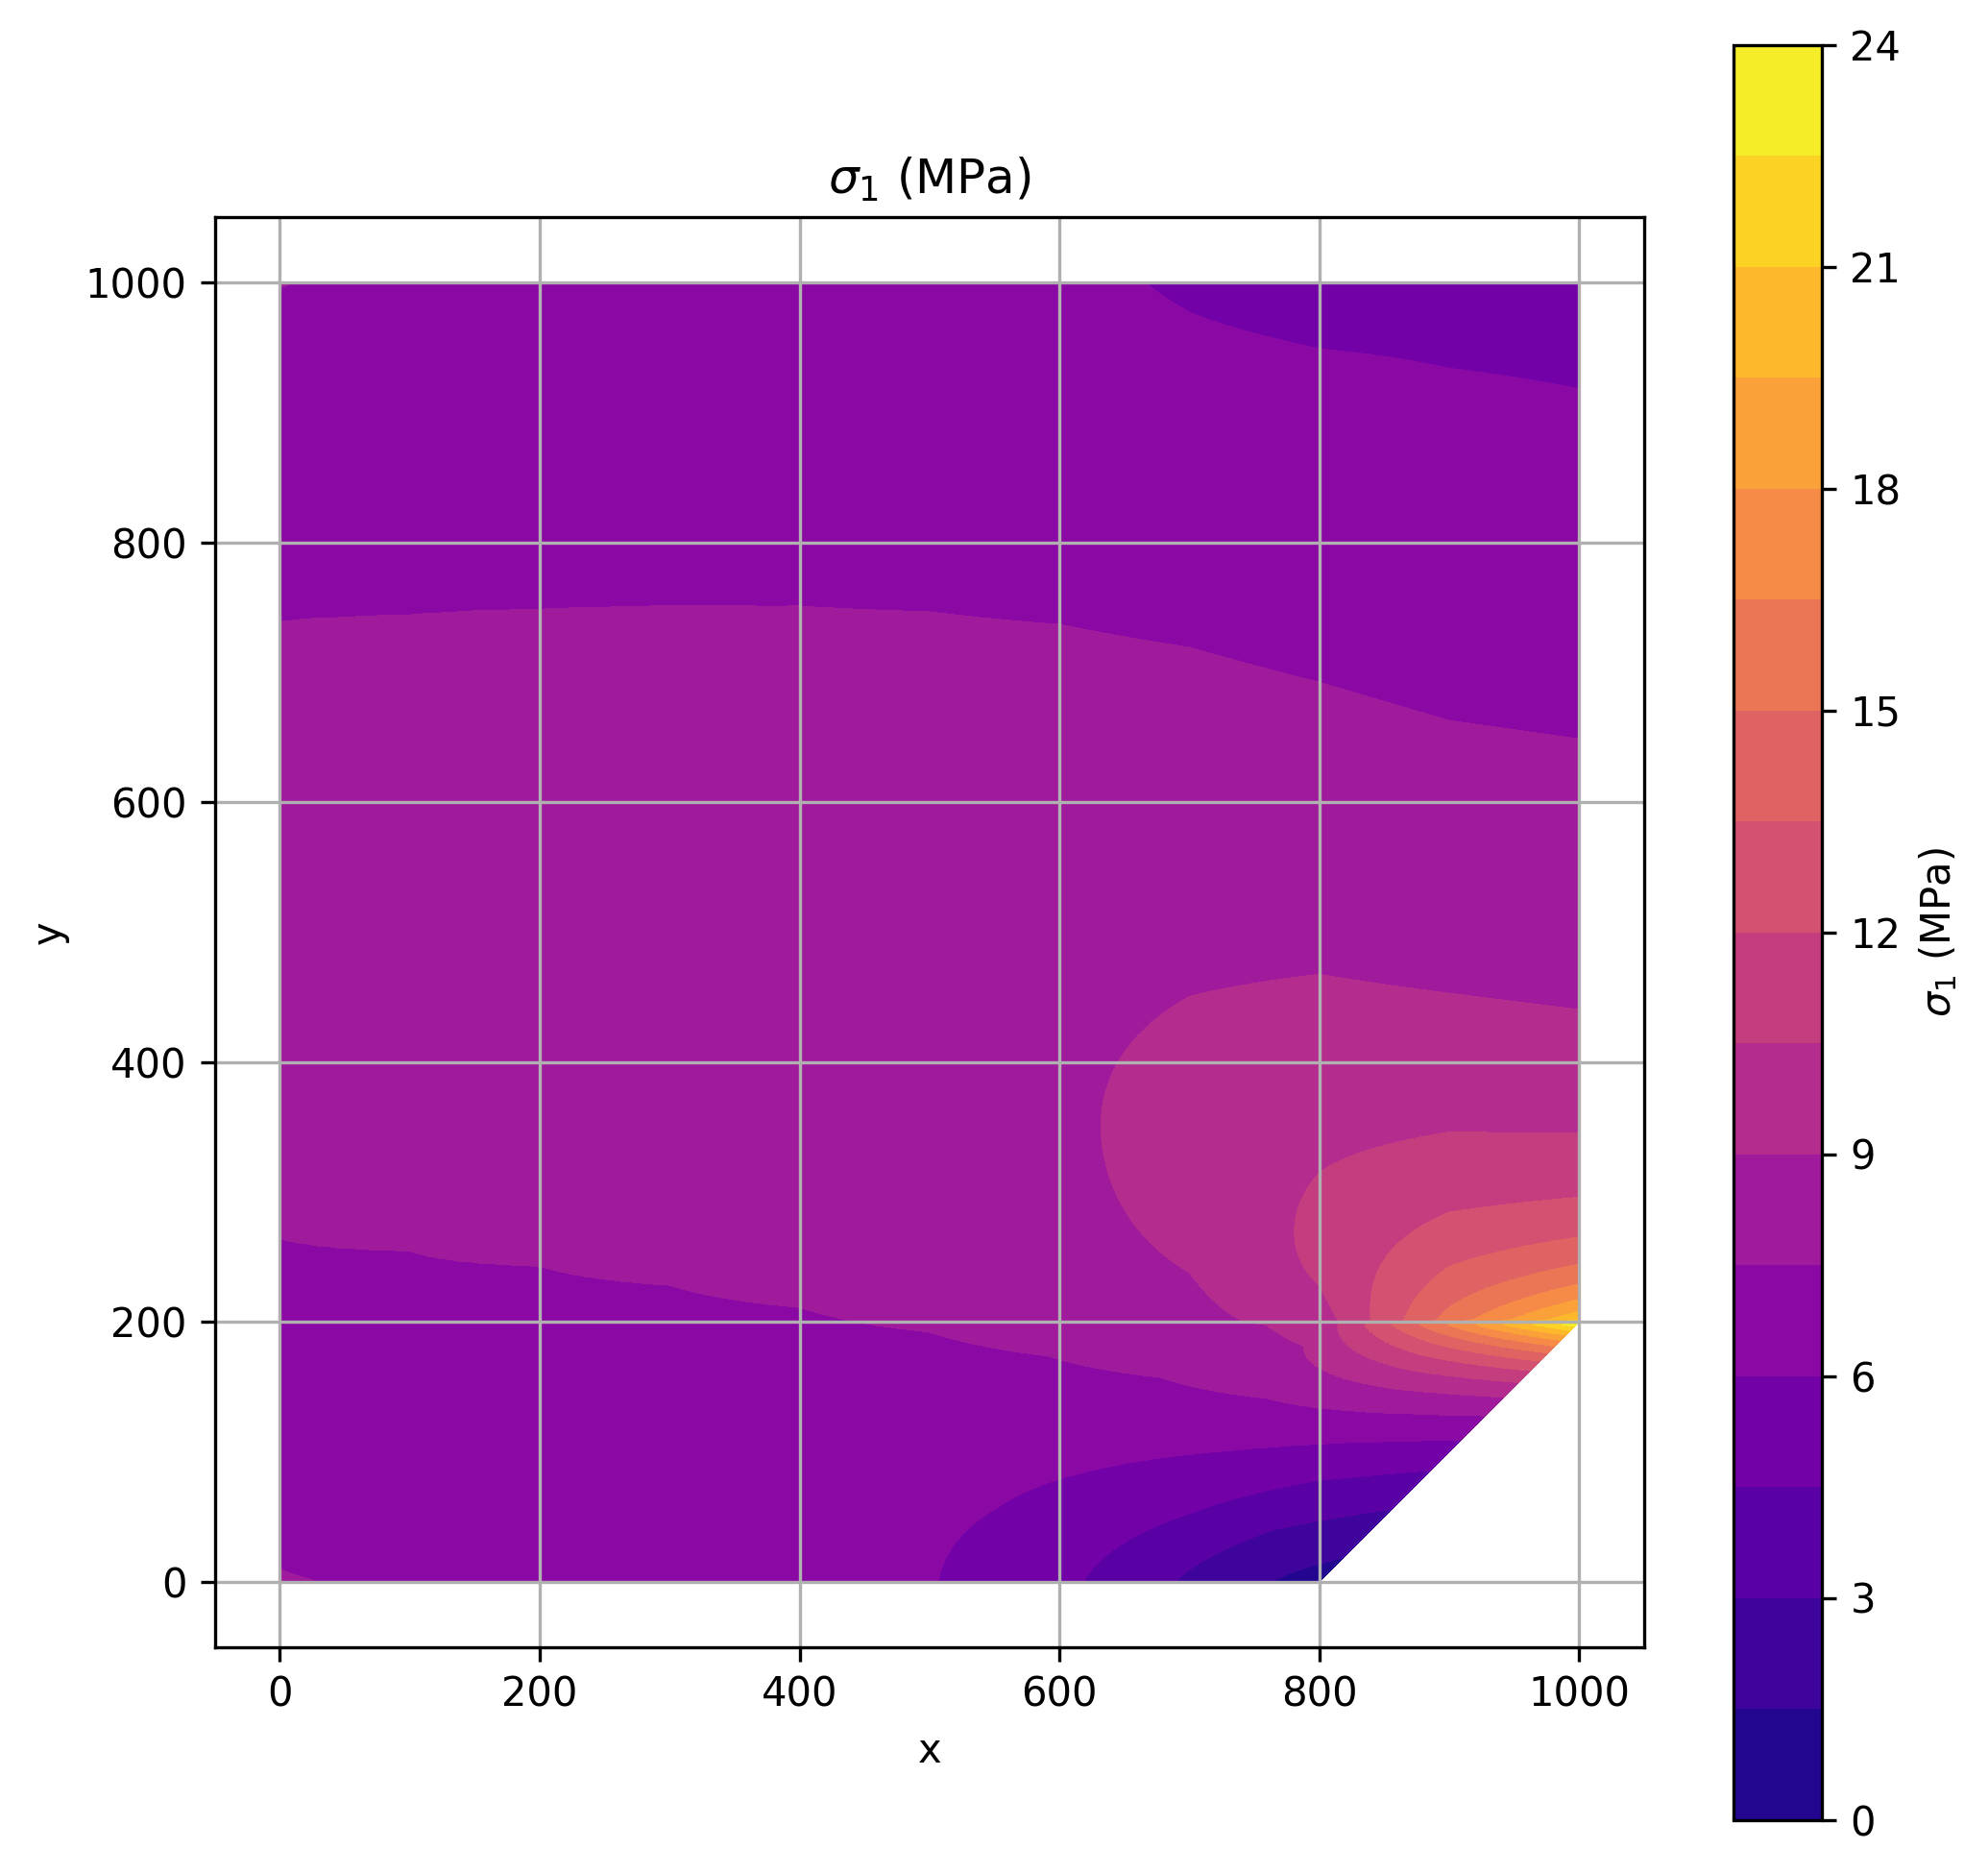
\includegraphics[width=\textwidth]{GRAFICOS/Quad4/2mm_global/resultados - sigma_1.png}
    \caption{Global mesh refinement - $h=2mm$}
    \label{fig:img1}
  \end{subfigure}
  \hfill
  \begin{subfigure}[b]{0.45\textwidth}
    \centering
    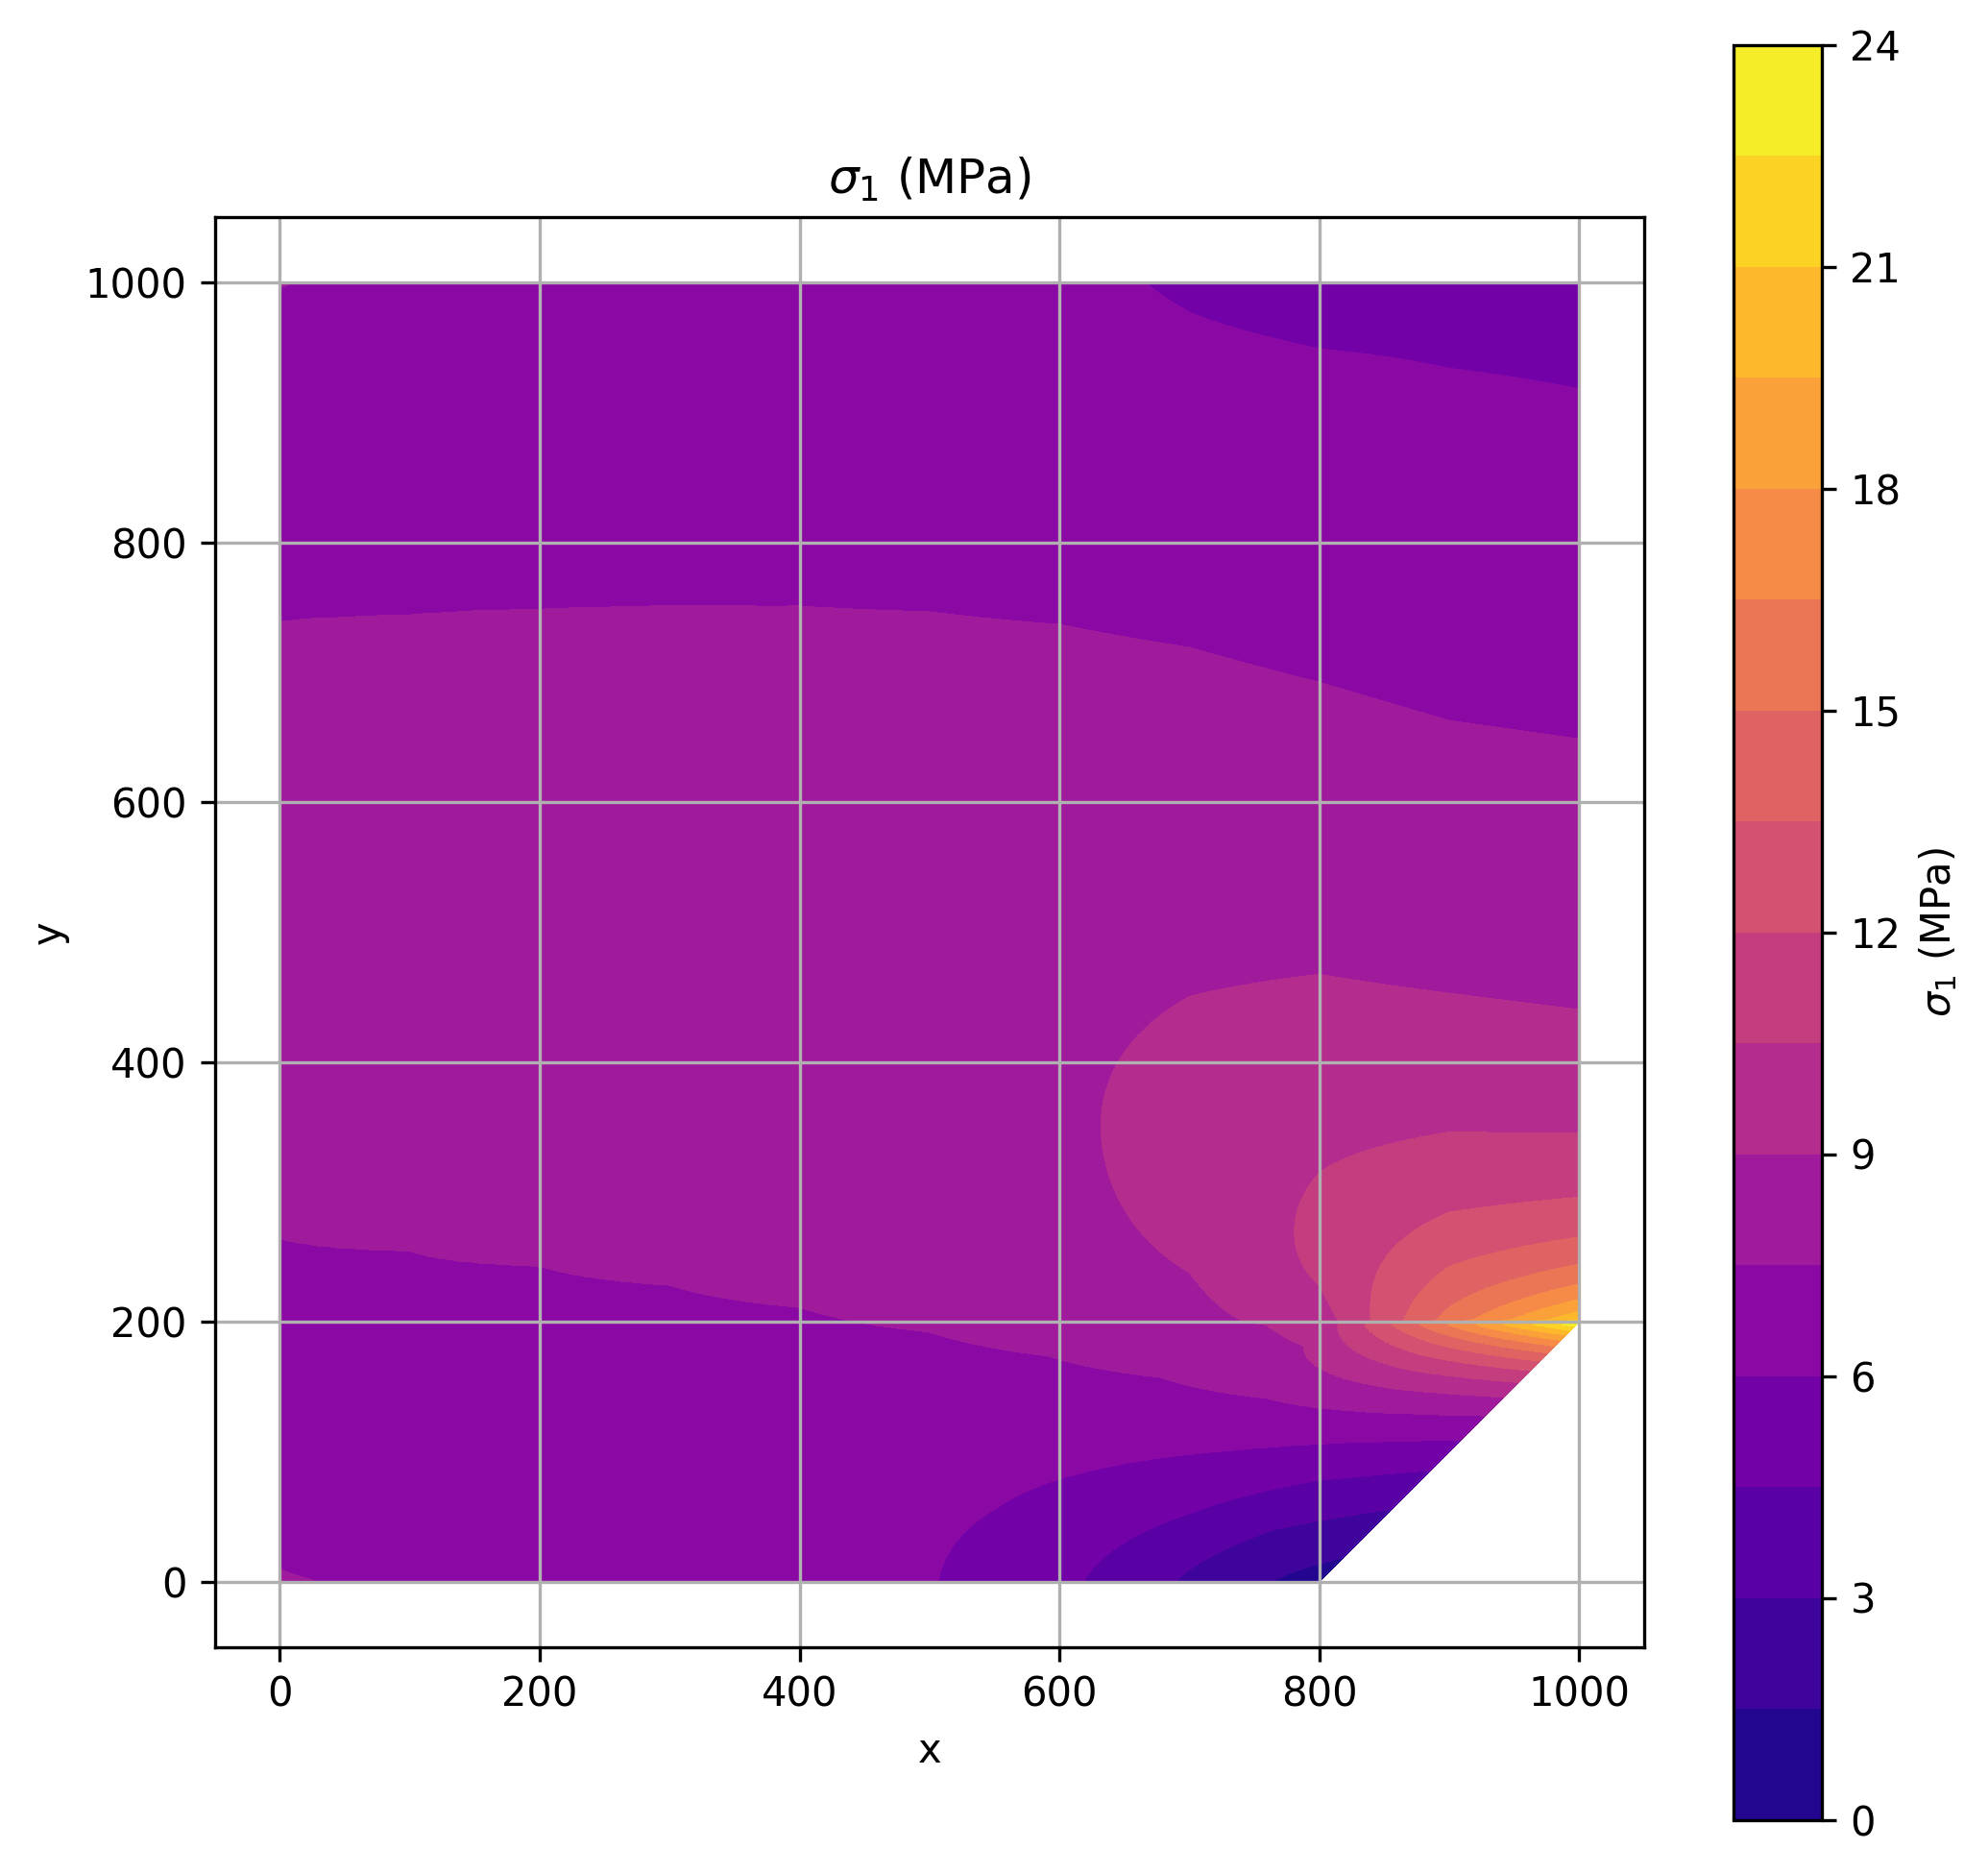
\includegraphics[width=\textwidth]{GRAFICOS/Quad4/2mm_global/resultados - sigma_1.png}
    \caption{Local mesh refinement - $h=2mm$}
    \label{fig:img2}
  \end{subfigure}
\end{figure}

\begin{figure}[H]
  \centering
  \begin{subfigure}[b]{0.45\textwidth}
    \centering
    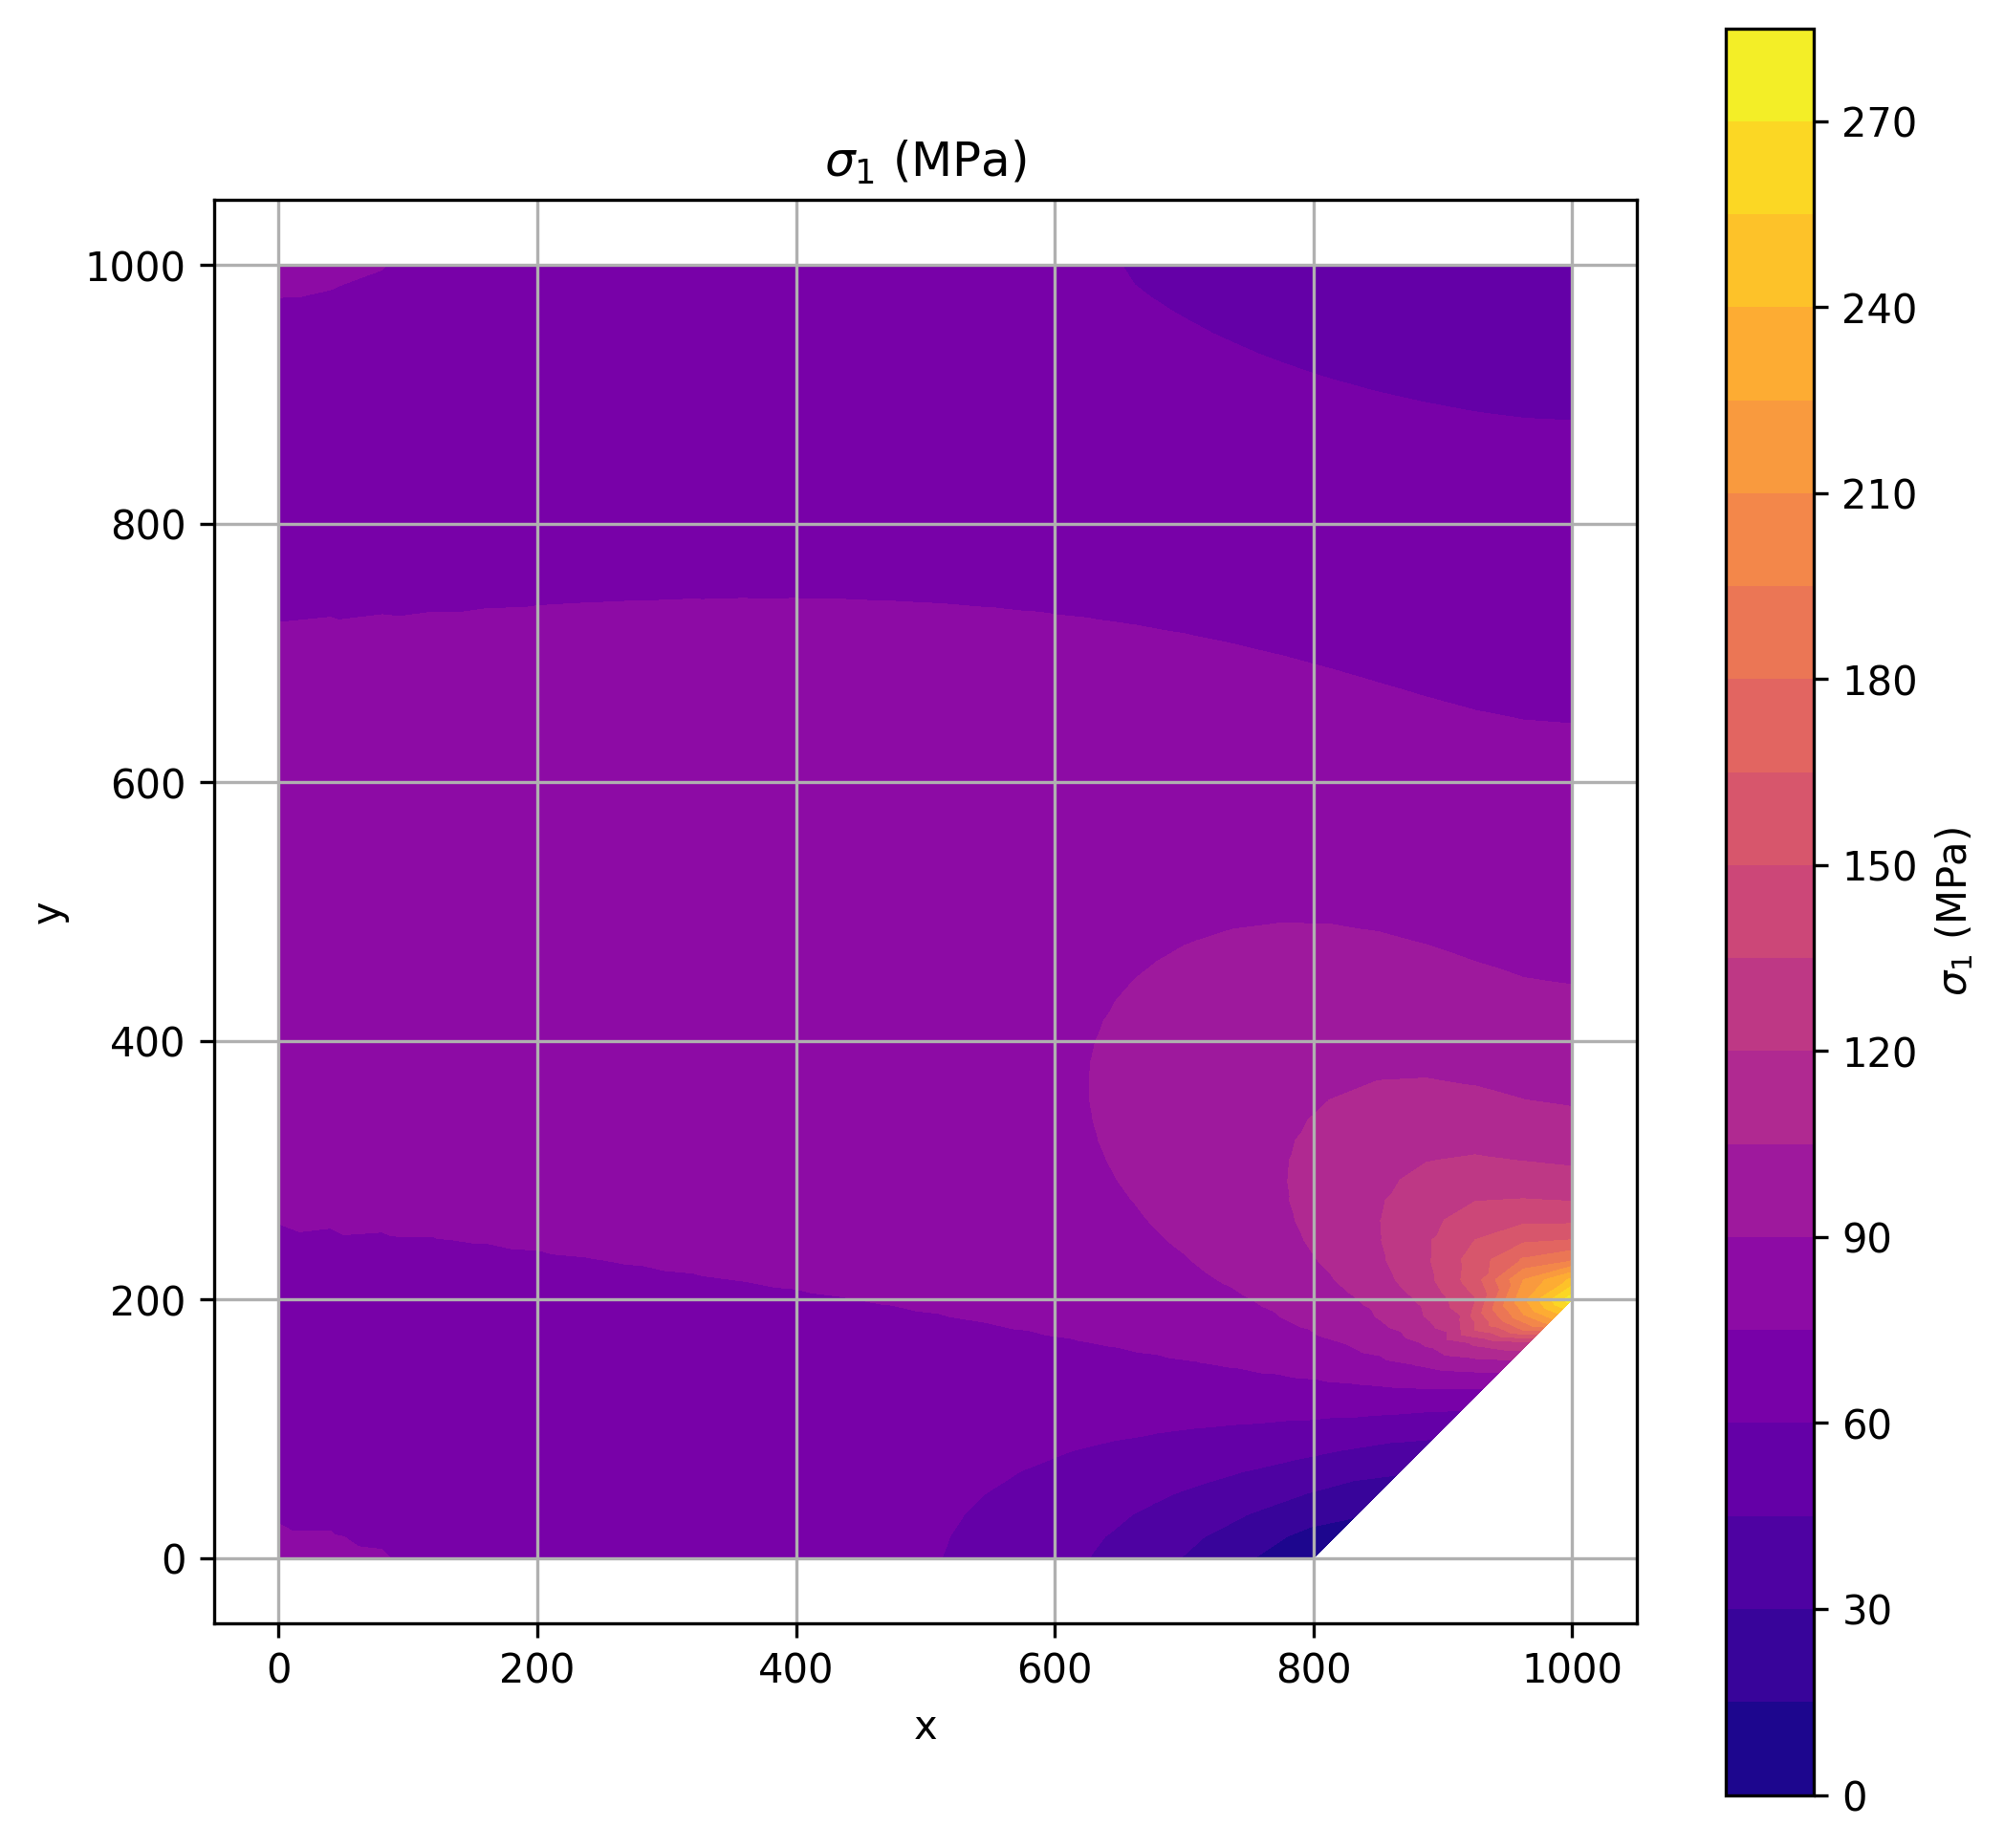
\includegraphics[width=\textwidth]{GRAFICOS/Quad4/1.75mm_global/resultados - sigma_1.png}
    \caption{Global mesh refinement - $h=1.75mm$}
    \label{fig:img11}
  \end{subfigure}
  \hfill
  \begin{subfigure}[b]{0.45\textwidth}
    \centering
    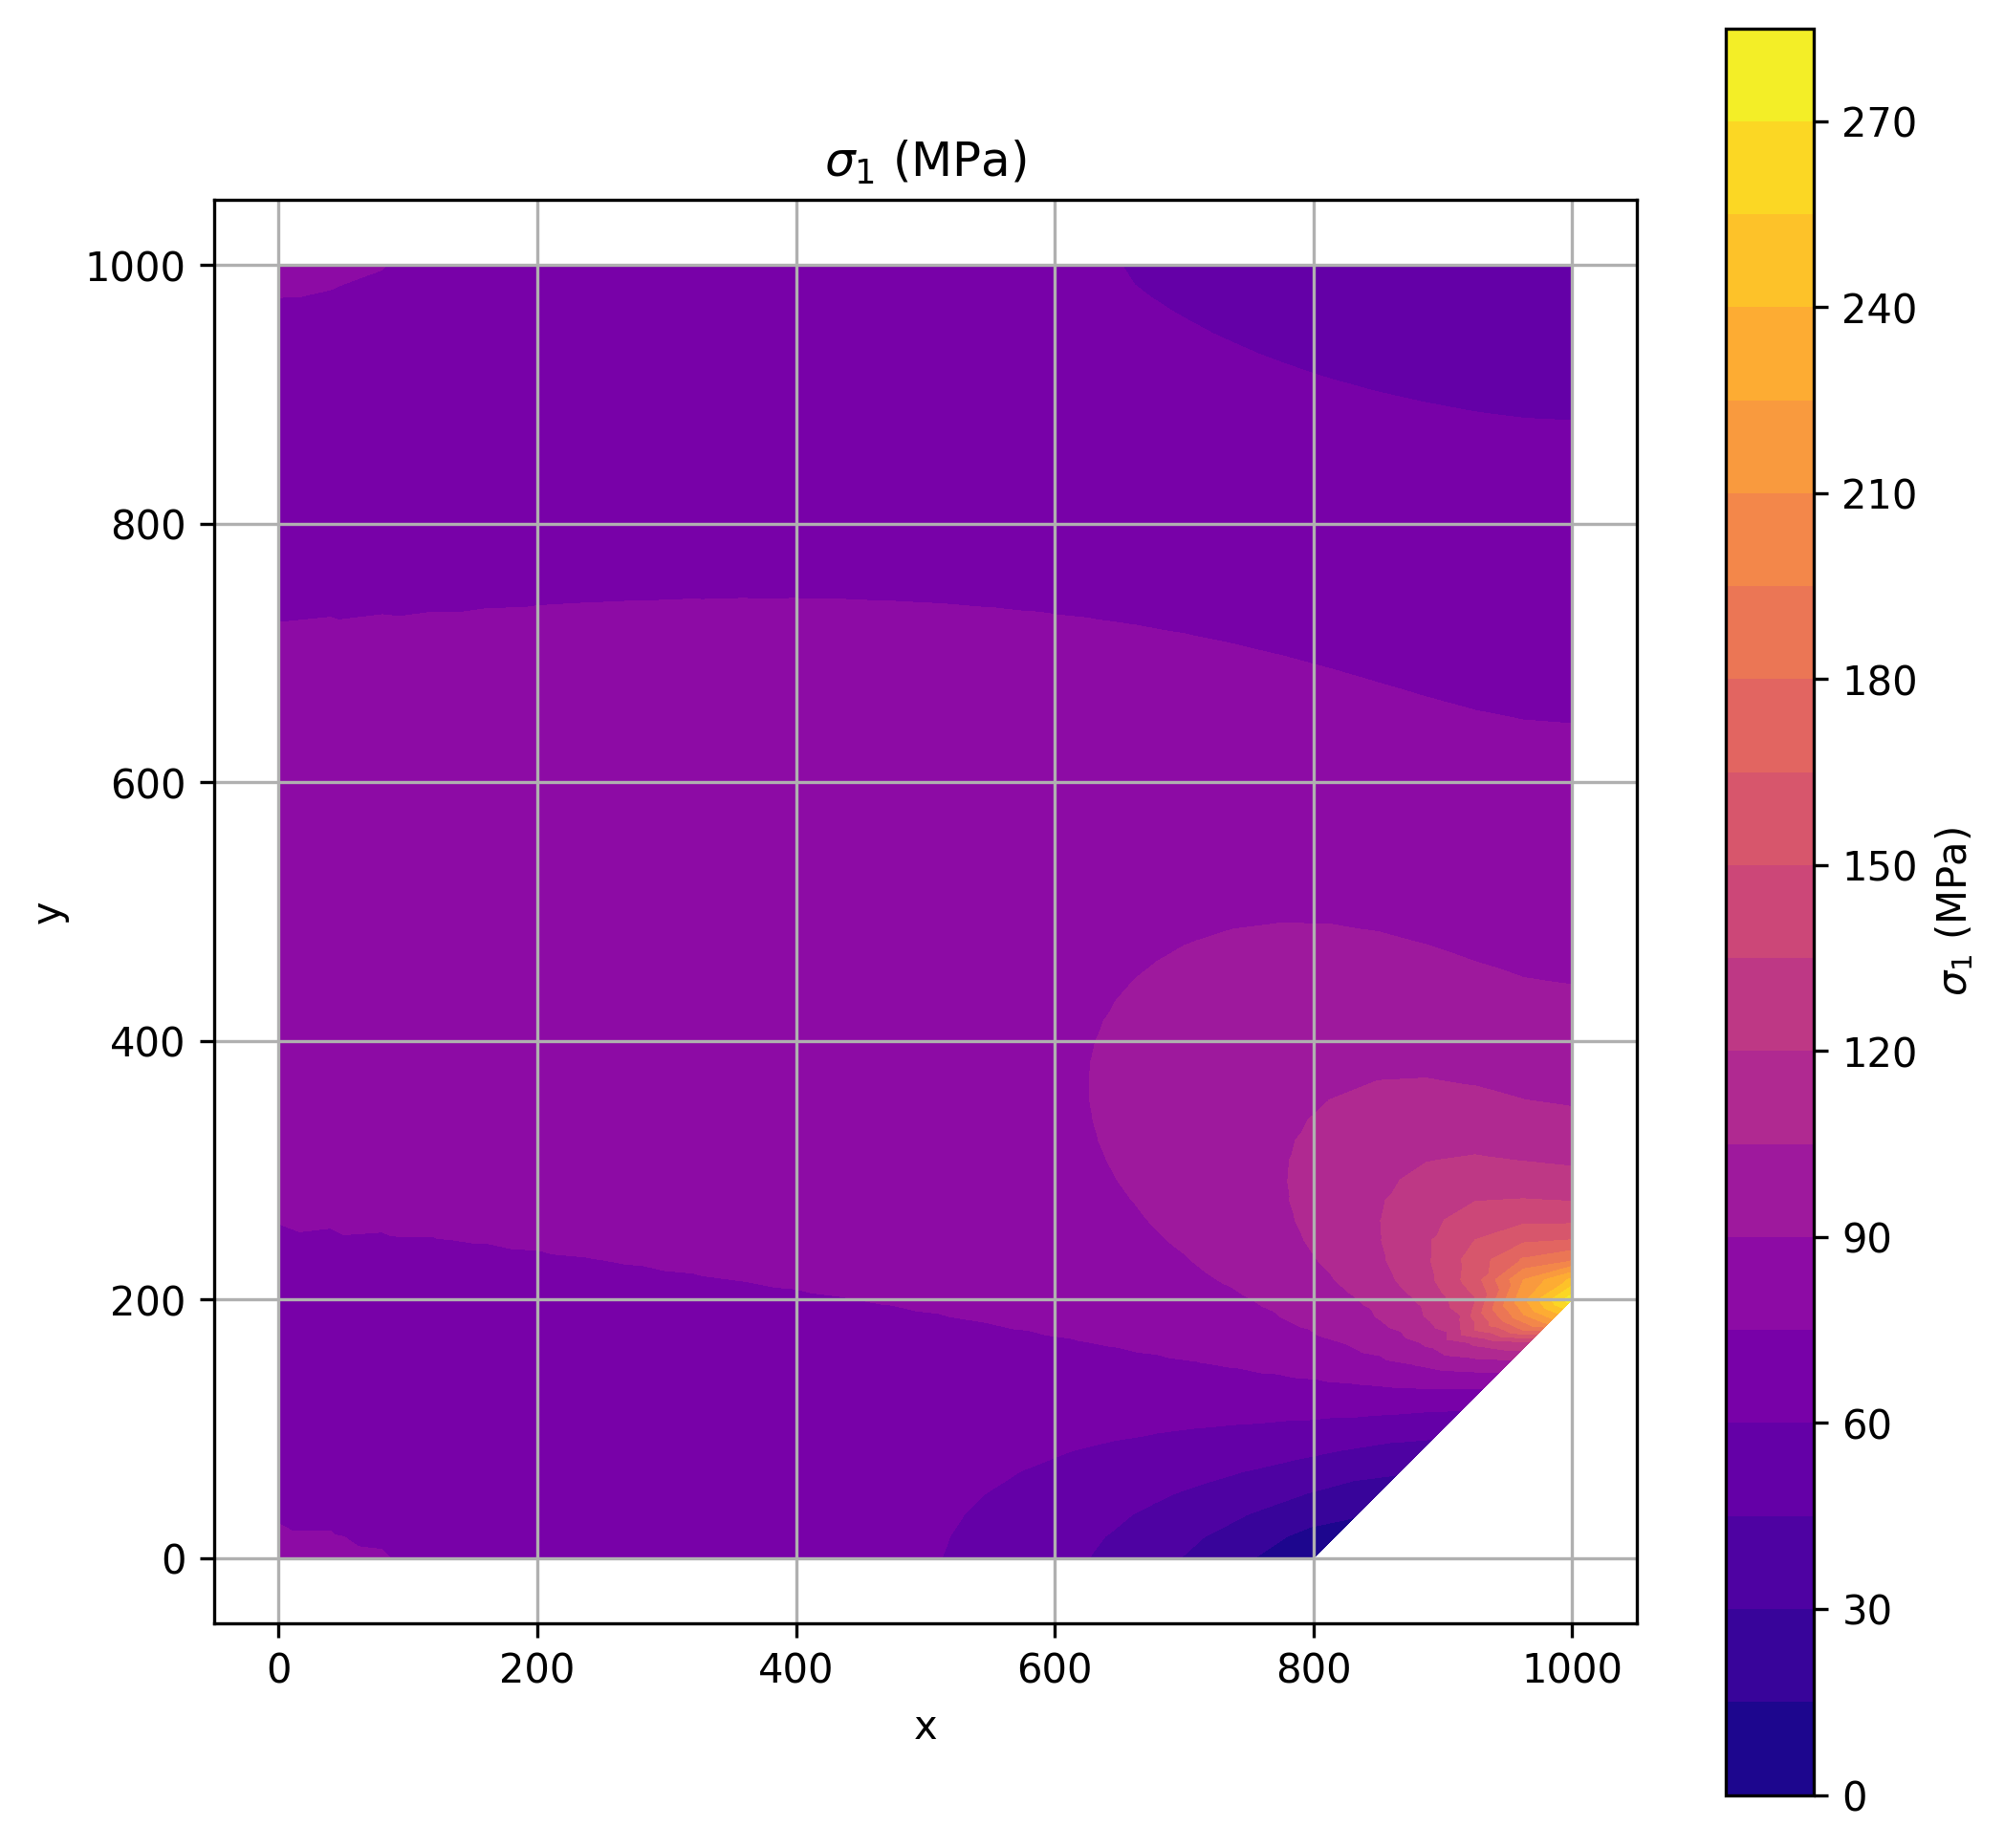
\includegraphics[width=\textwidth]{GRAFICOS/Quad4/1.75mm_global/resultados - sigma_1.png}
    \caption{Local mesh refinement - $h=1.75mm$}
    \label{fig:img21}
  \end{subfigure}
\end{figure}

\begin{figure}[H]
  \centering
  \begin{subfigure}[b]{0.45\textwidth}
    \centering
    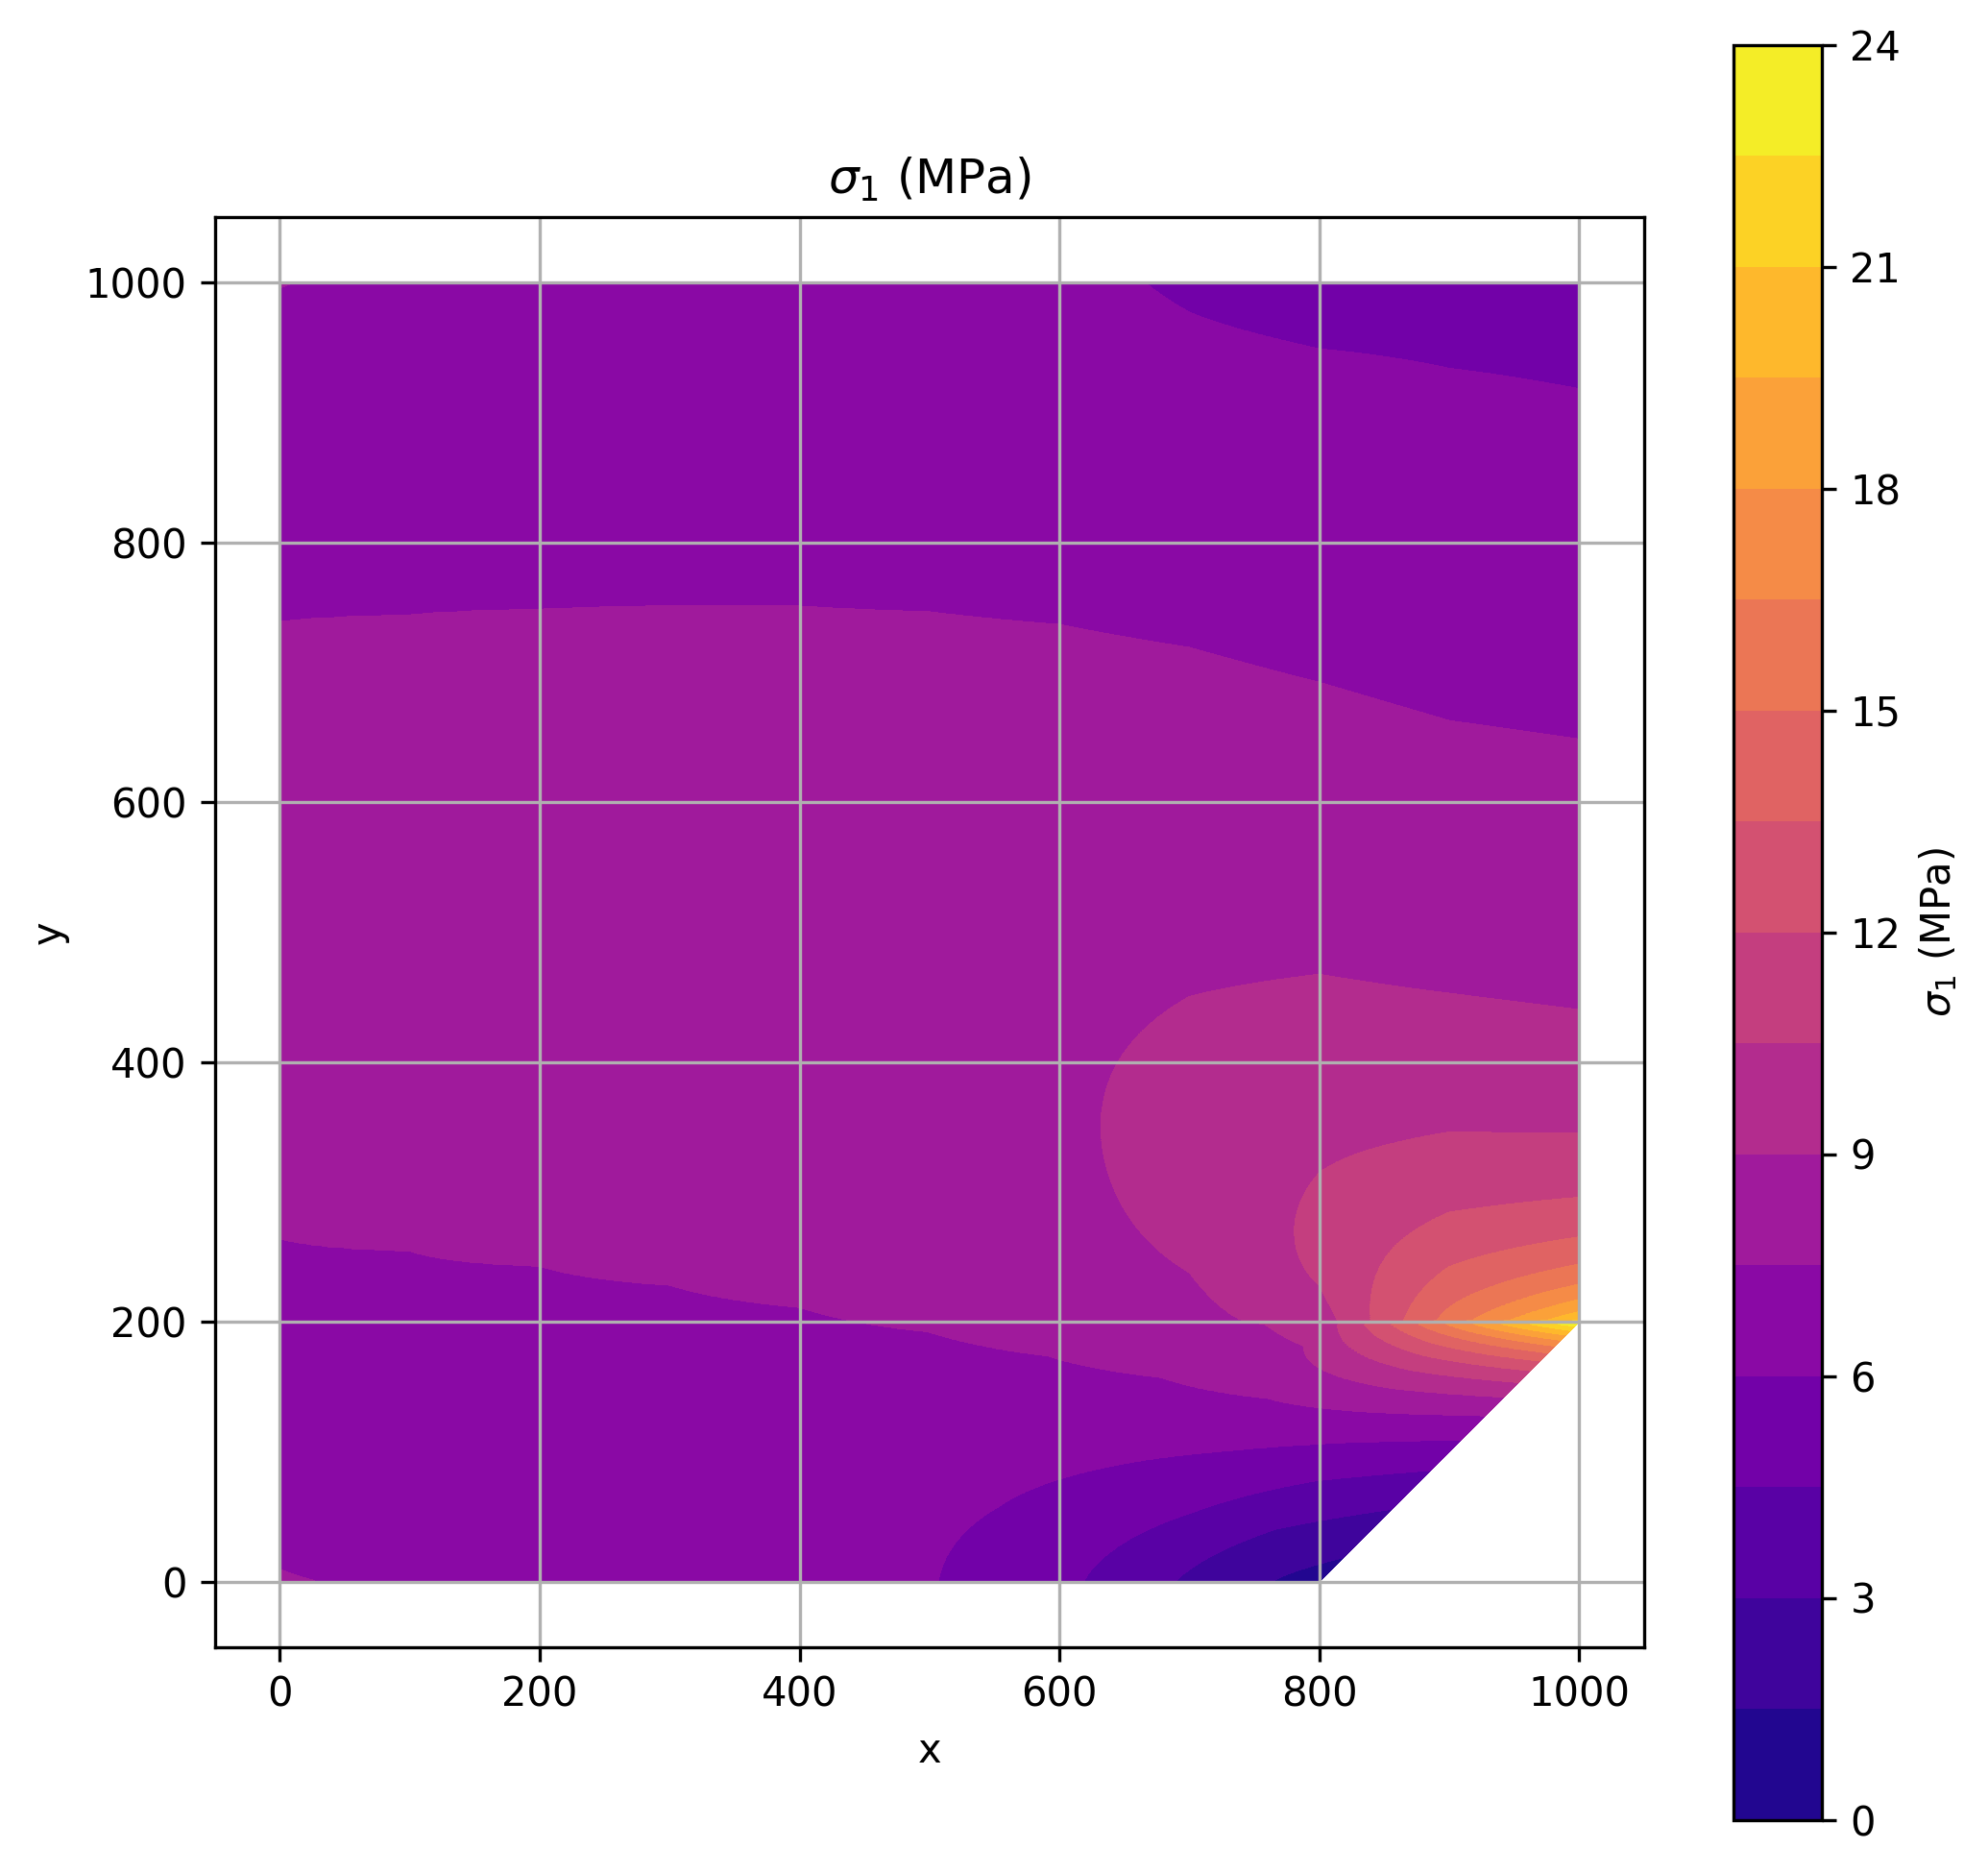
\includegraphics[width=\textwidth]{GRAFICOS/Quad4/1.5mm_global/resultados - sigma_1.png}
    \caption{Global mesh refinement - $h=1.5mm$}
    \label{fig:img12}
  \end{subfigure}
  \hfill
  \begin{subfigure}[b]{0.45\textwidth}
    \centering
    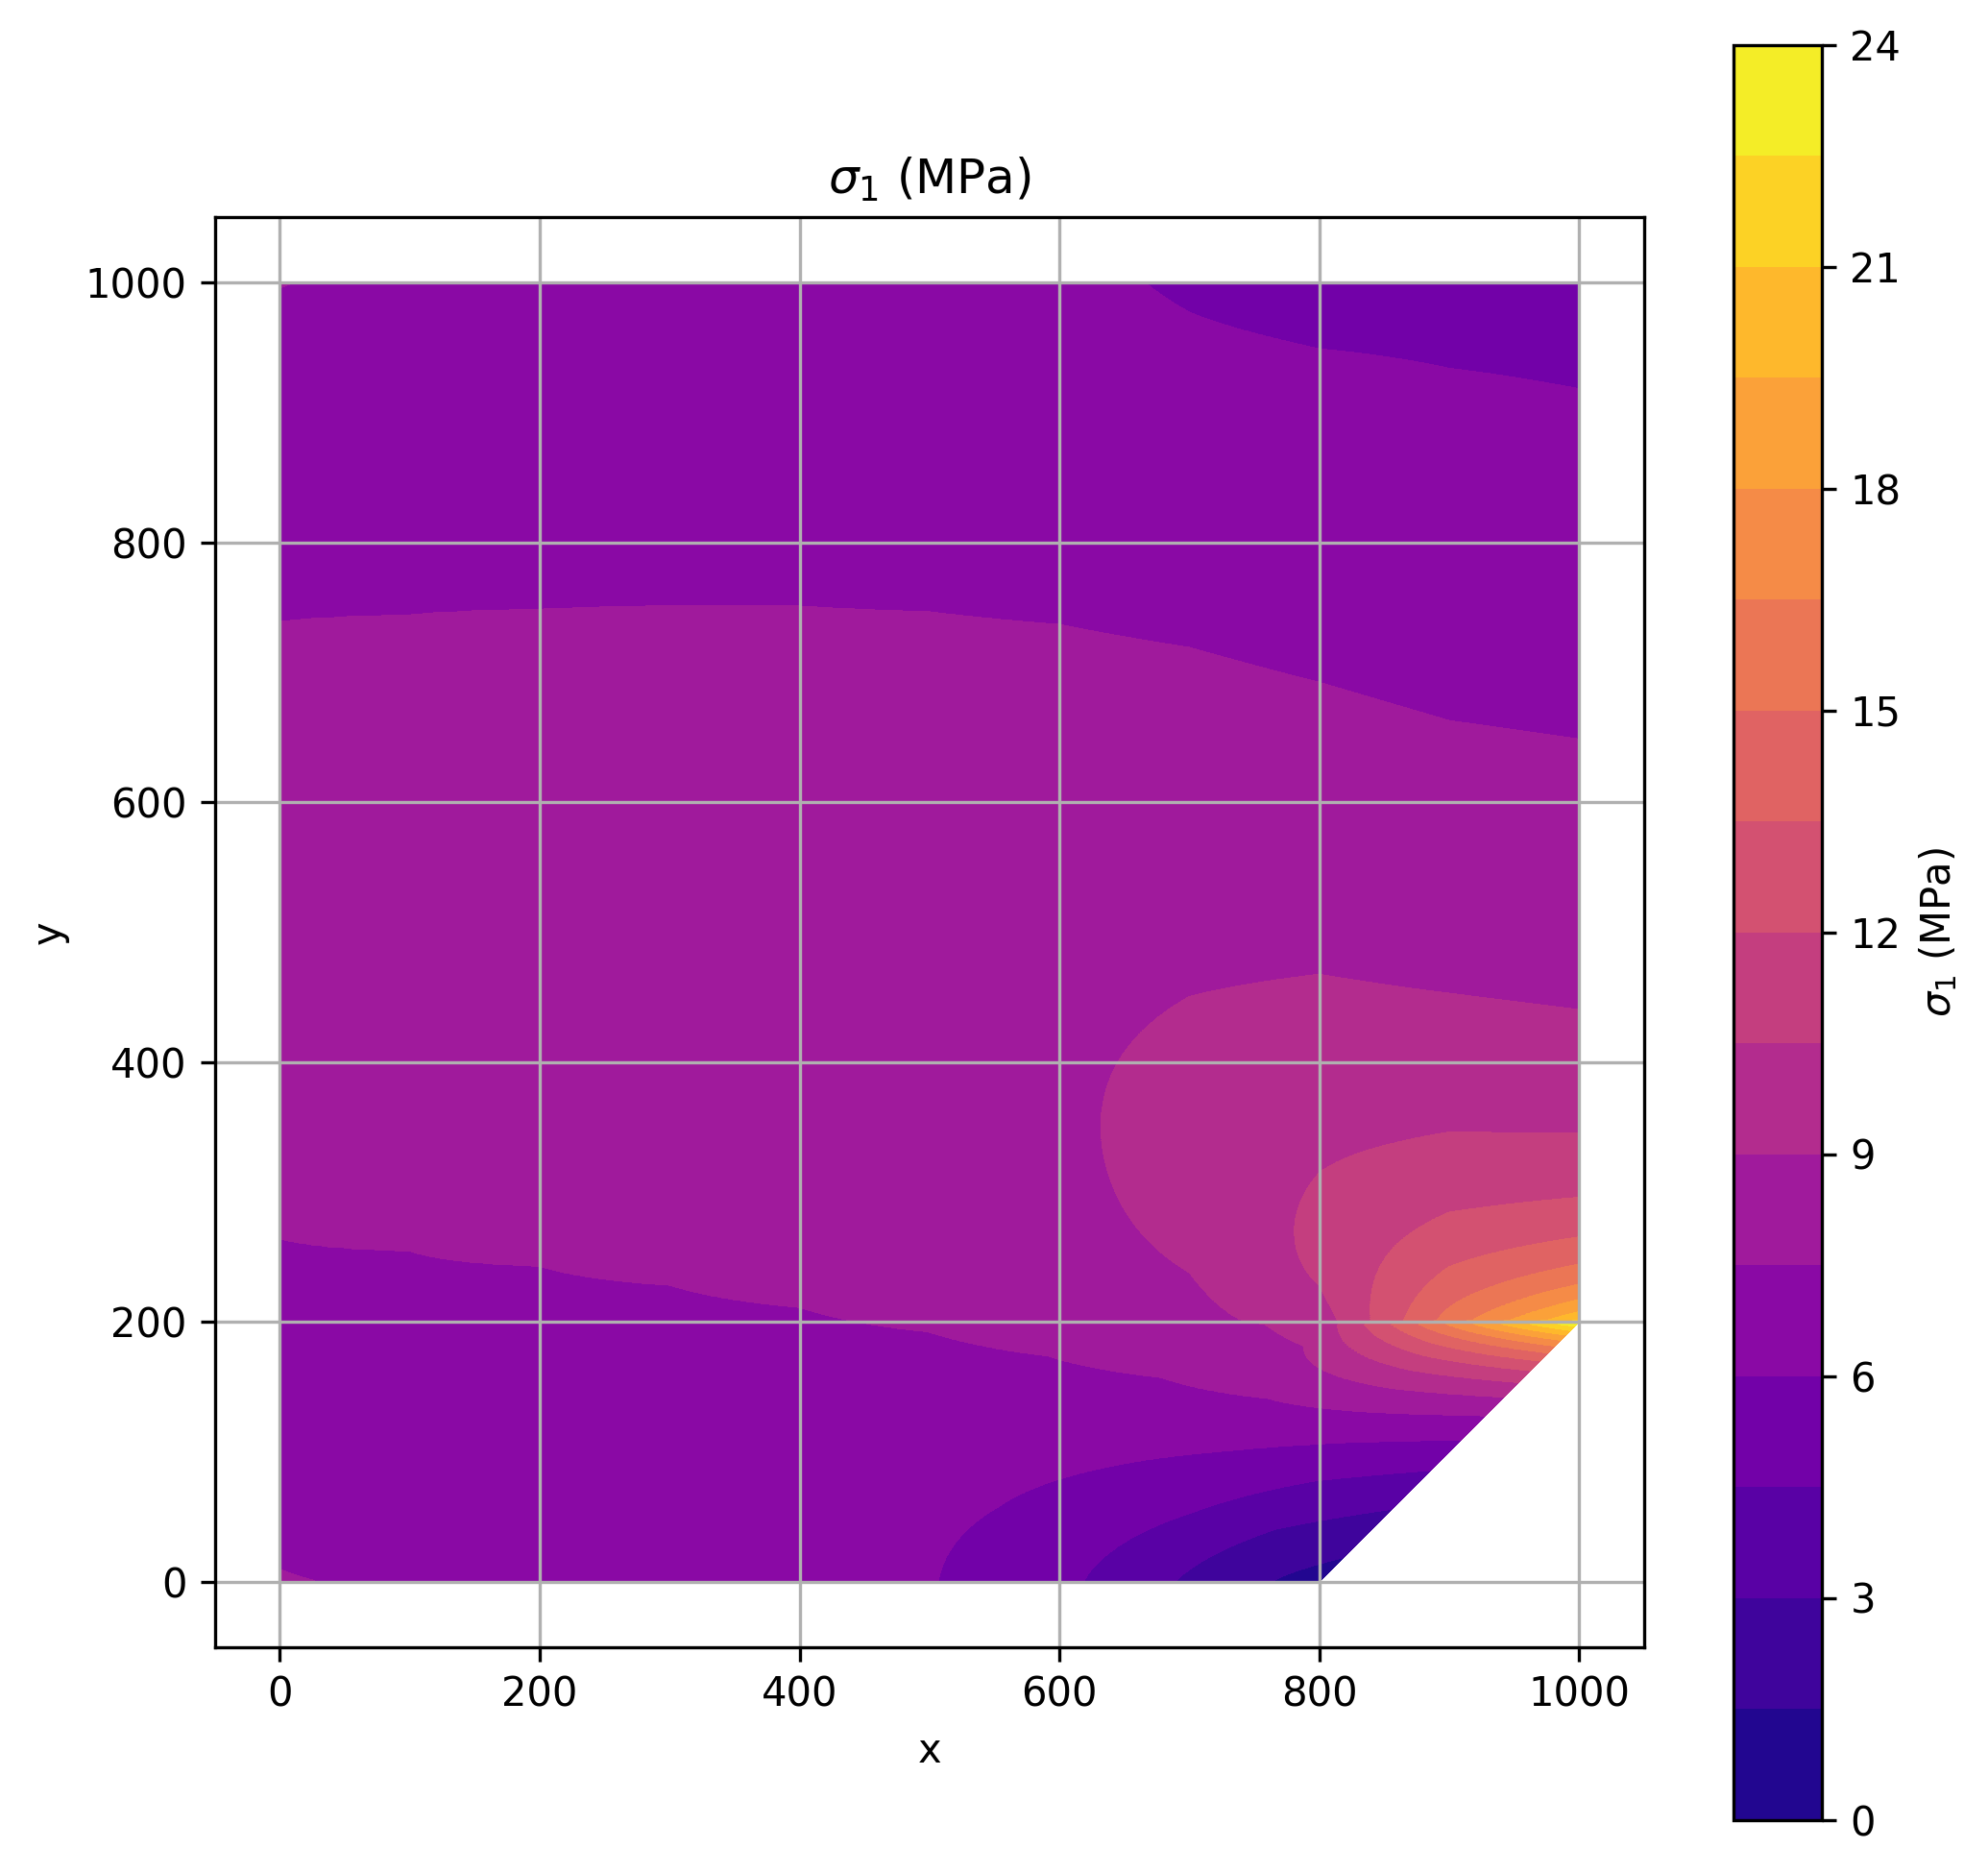
\includegraphics[width=\textwidth]{GRAFICOS/Quad4/1.5mm_global/resultados - sigma_1.png}
    \caption{Local mesh refinement - $h=1.5mm$}
    \label{fig:img22}
  \end{subfigure}
\end{figure}

\begin{figure}[H]
  \centering
  \begin{subfigure}[b]{0.45\textwidth}
    \centering
    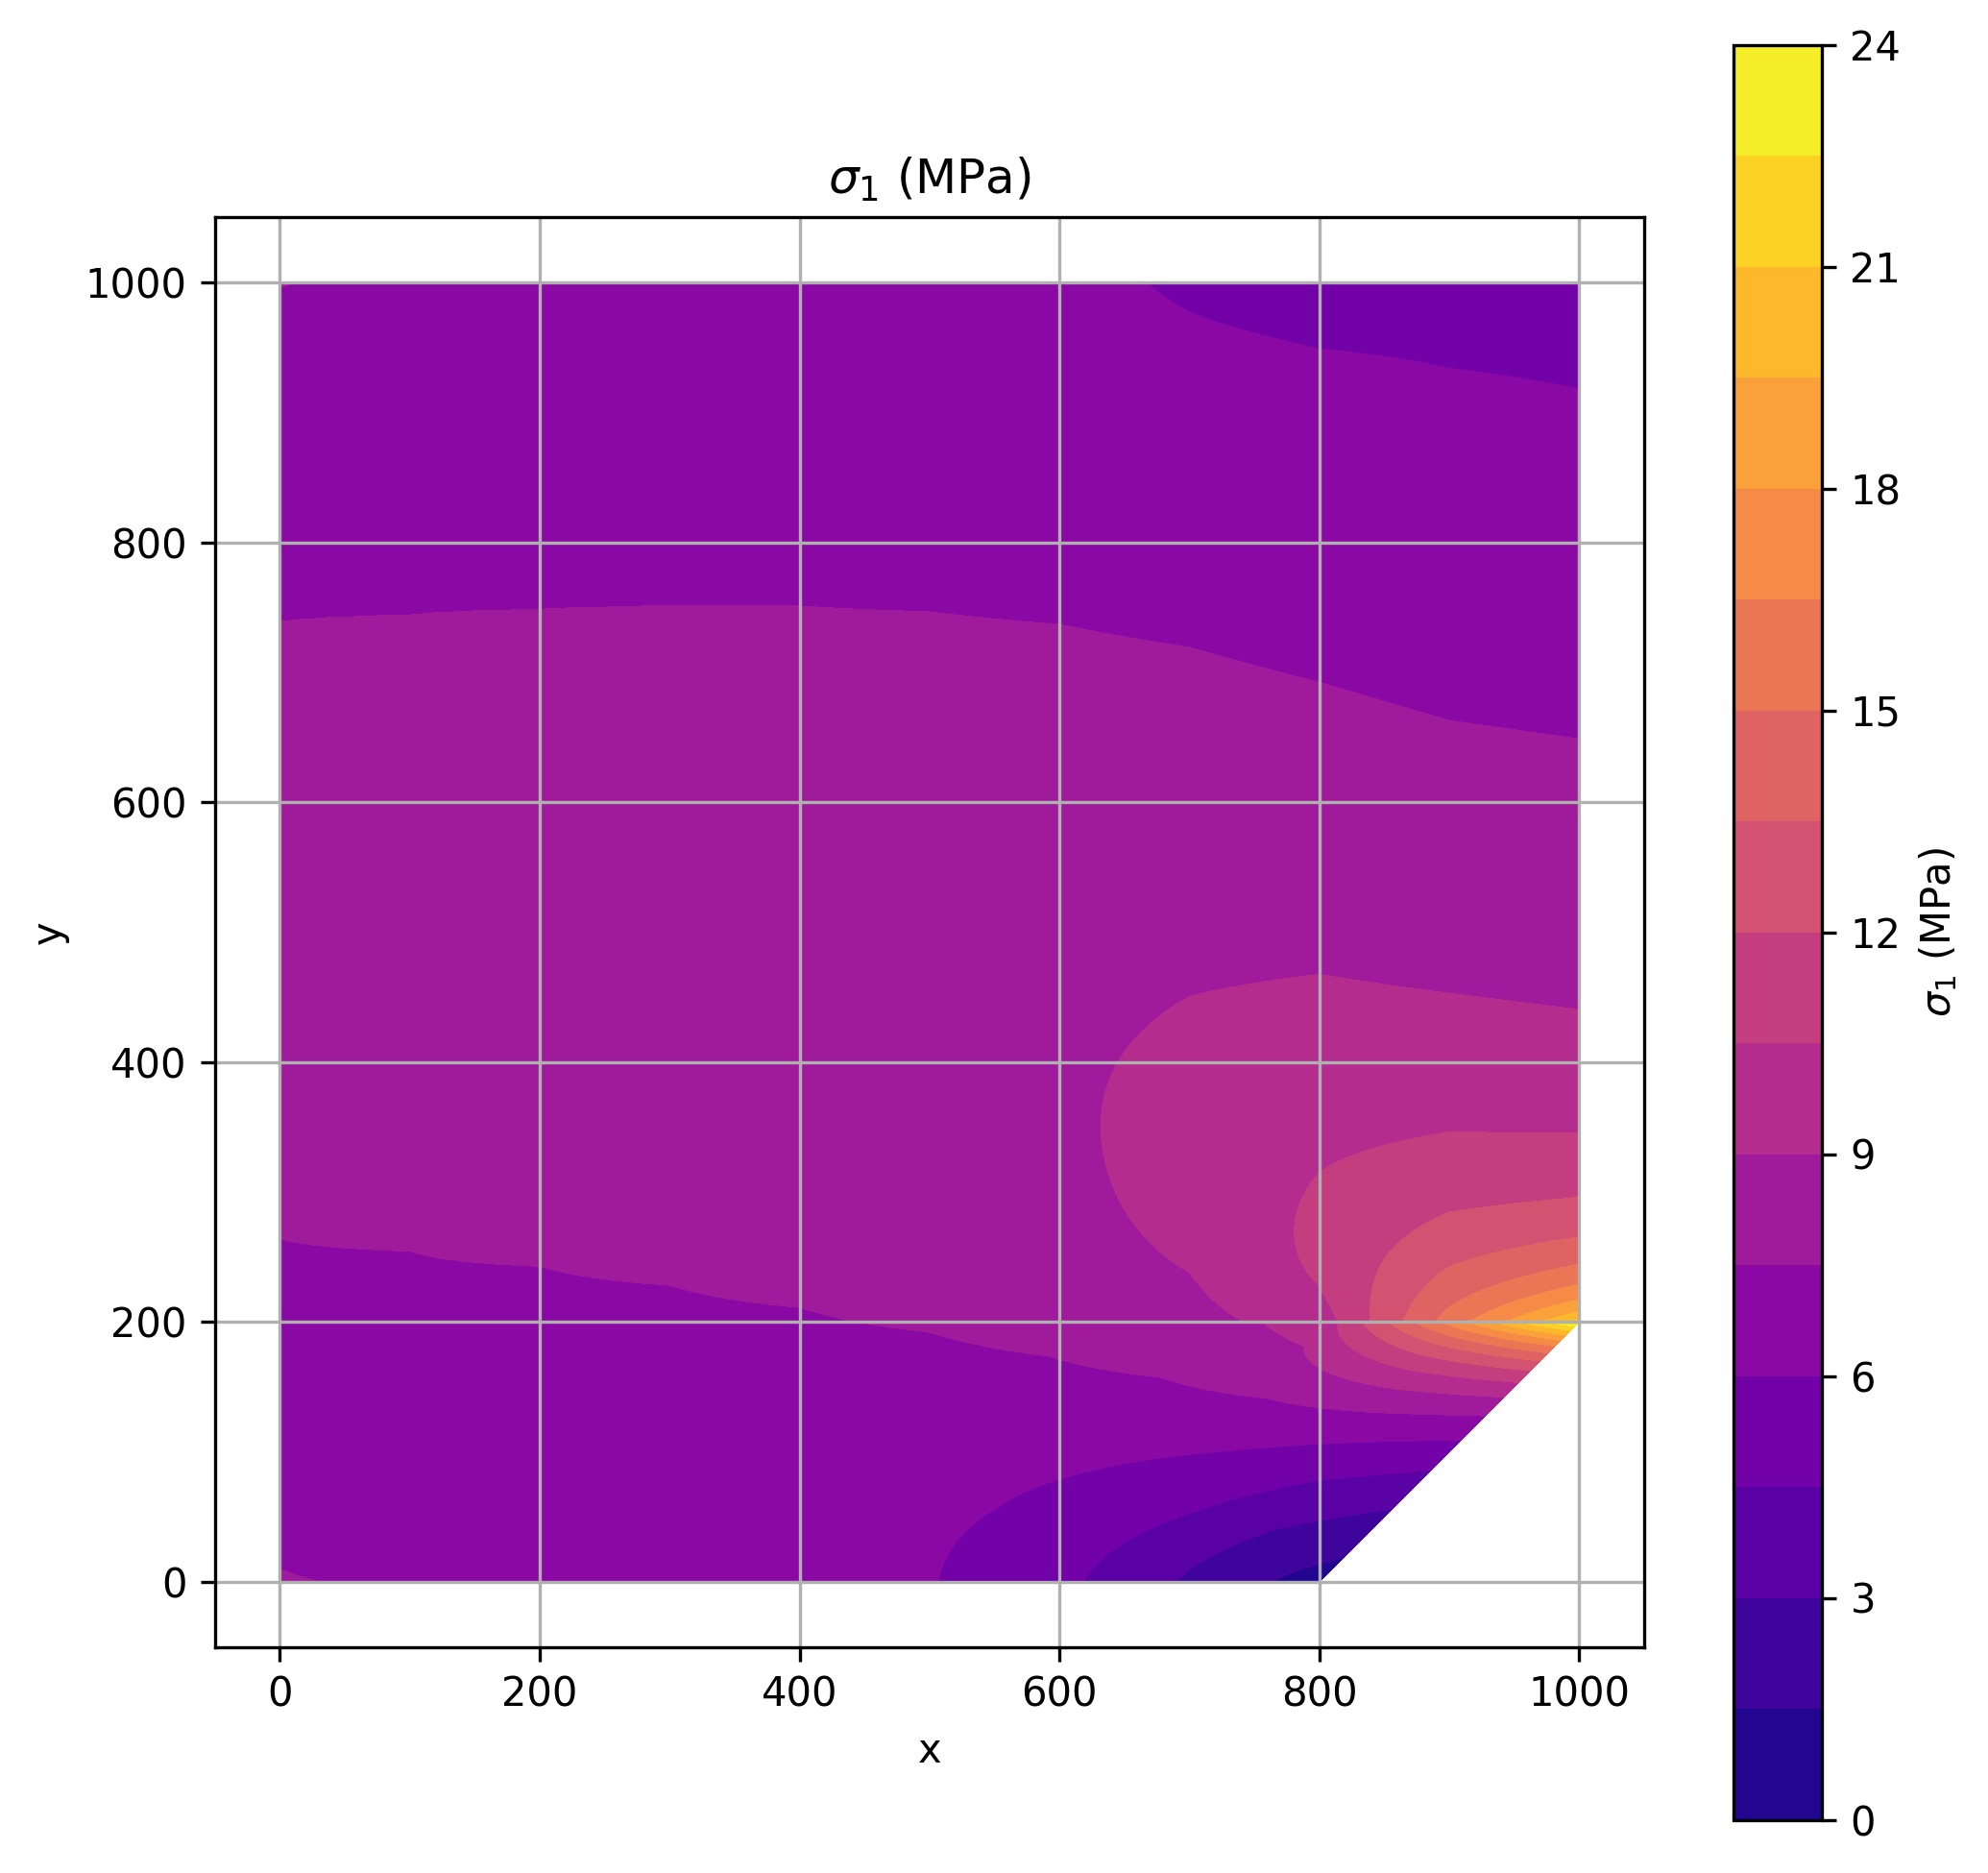
\includegraphics[width=\textwidth]{GRAFICOS/Quad4/1.25mm_global/resultados - sigma_1.png}
    \caption{Global mesh refinement - $h=1.25mm$}
    \label{fig:img13}
  \end{subfigure}
  \hfill
  \begin{subfigure}[b]{0.45\textwidth}
    \centering
    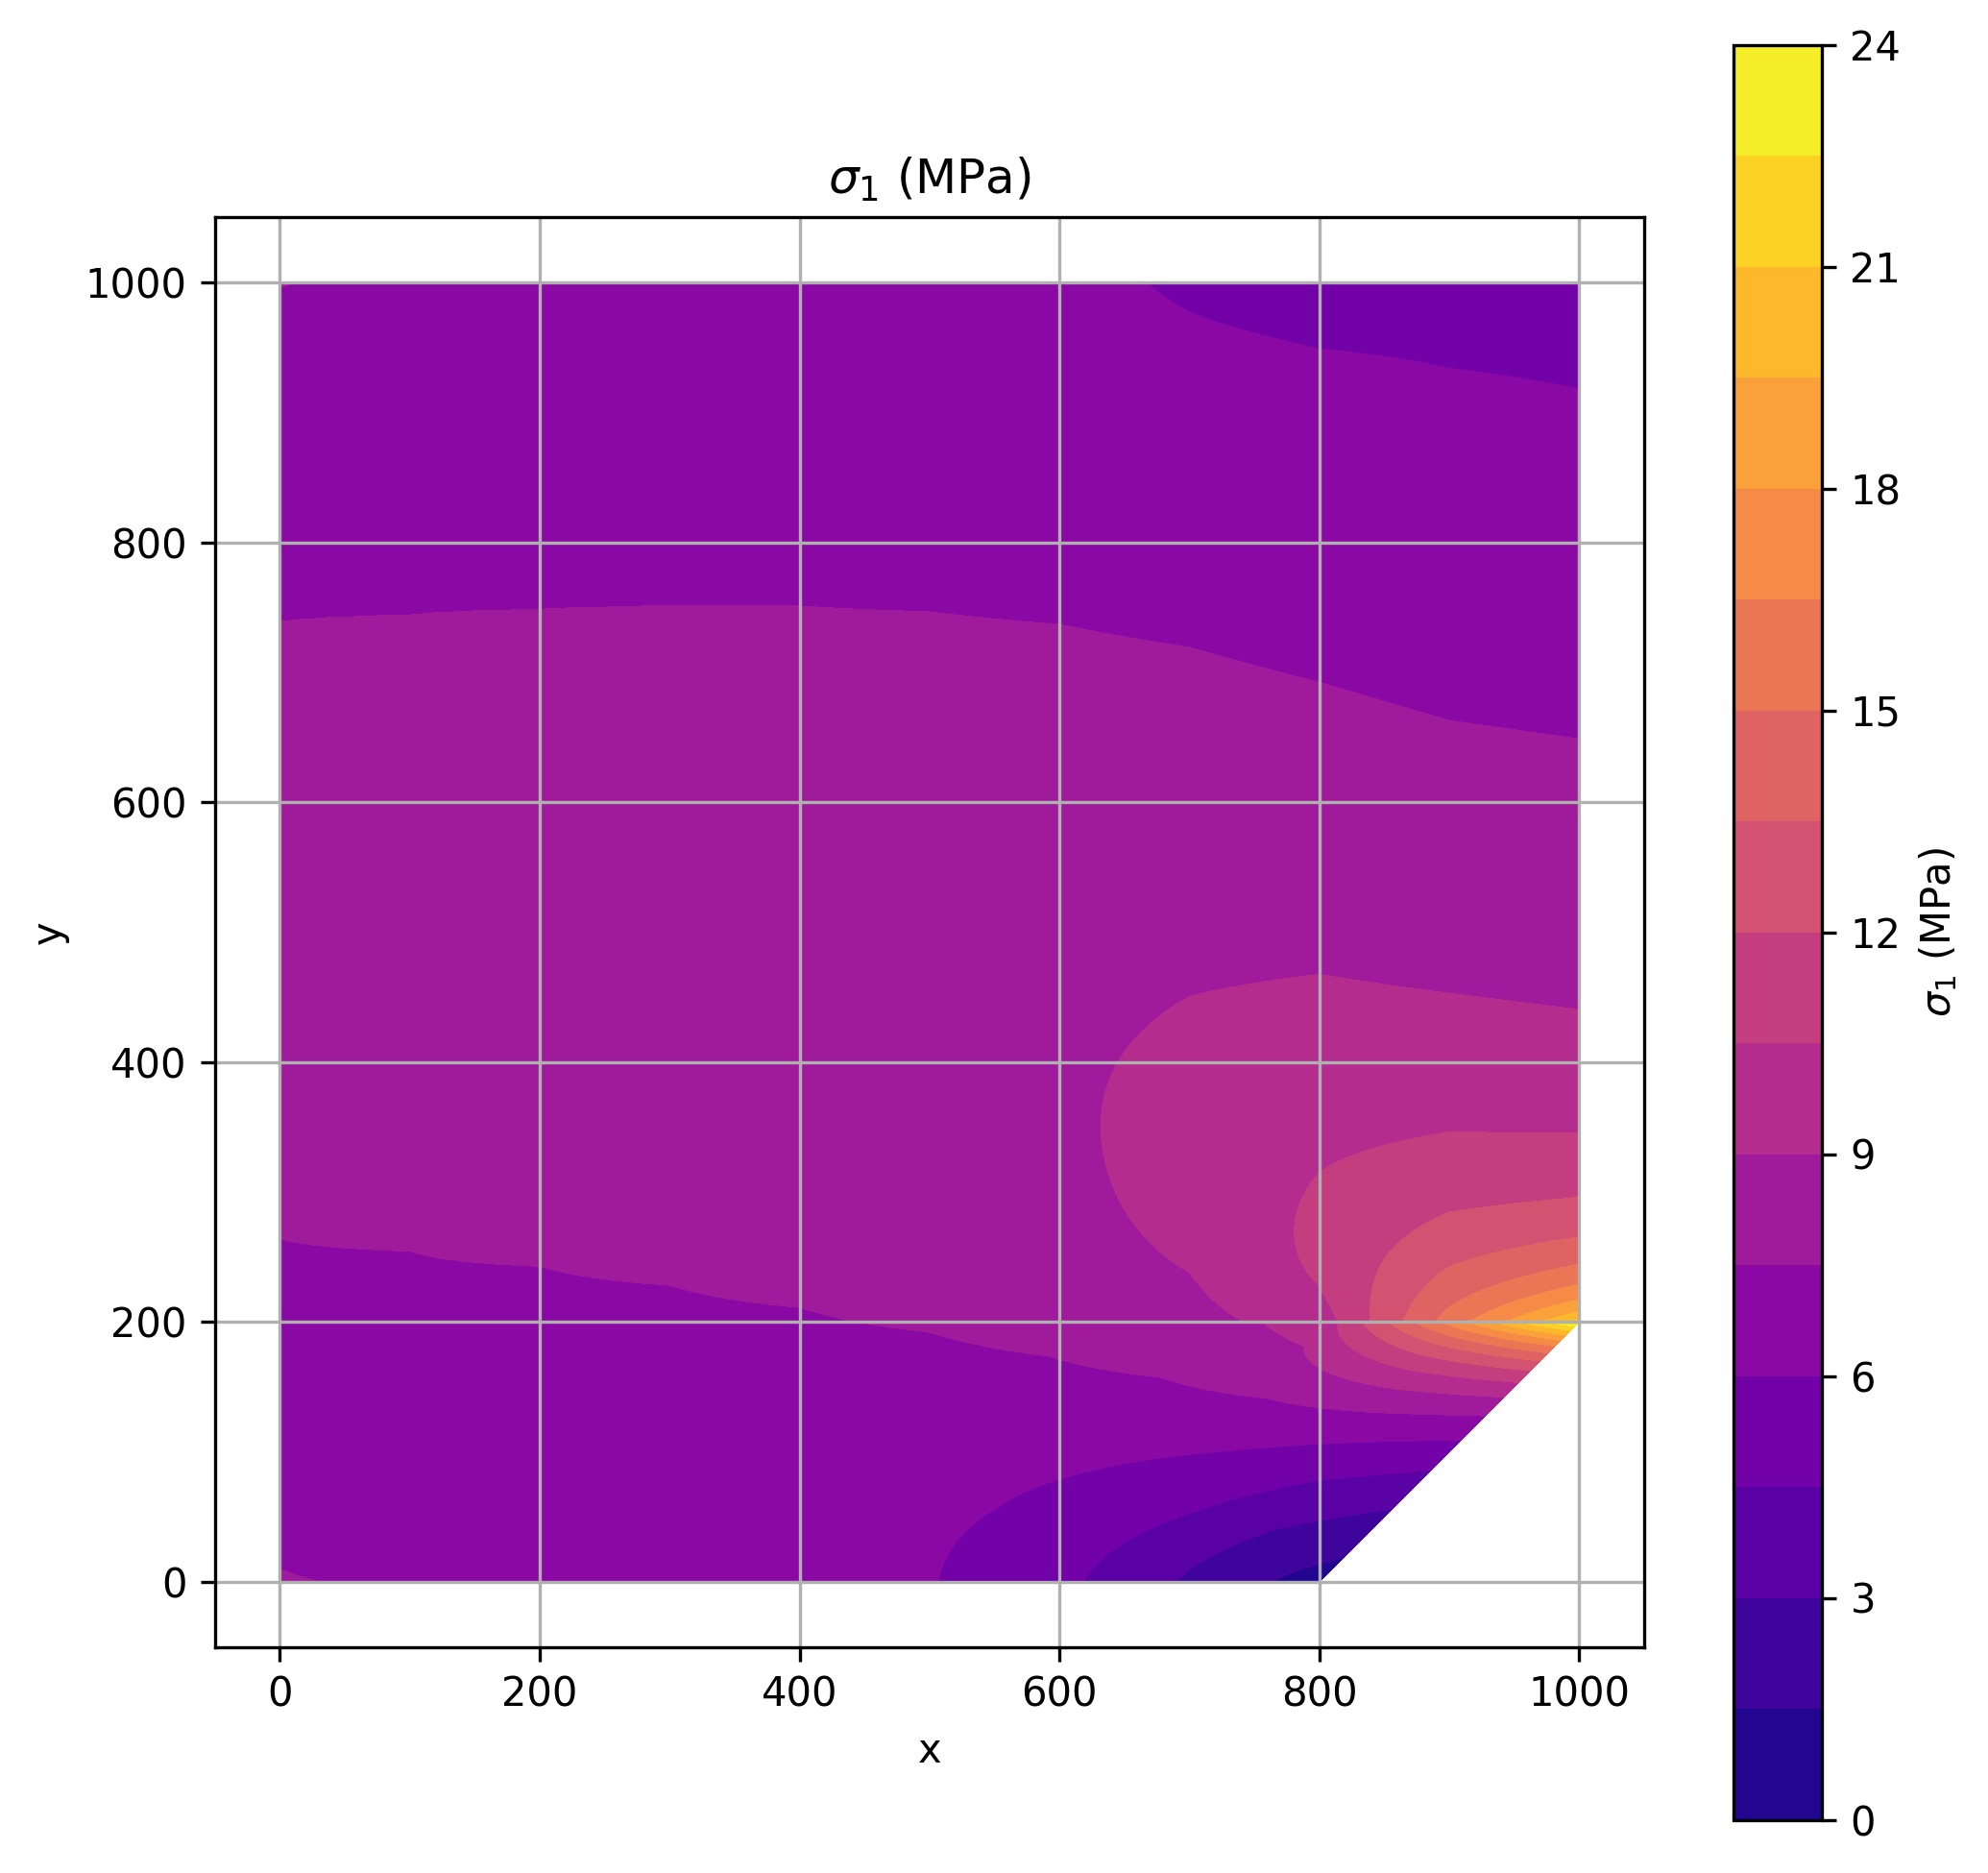
\includegraphics[width=\textwidth]{GRAFICOS/Quad4/1.25mm_global/resultados - sigma_1.png}
    \caption{Local mesh refinement - $h=1.25mm$}
    \label{fig:img23}
  \end{subfigure}
\end{figure}

\subsubsection{Quad9 Element}

In this section, the same procedure was followed, but increasing the order of the mesh elements to Quad9.

\begin{figure}[H]
  \centering
  \begin{subfigure}[b]{0.45\textwidth}
    \centering
    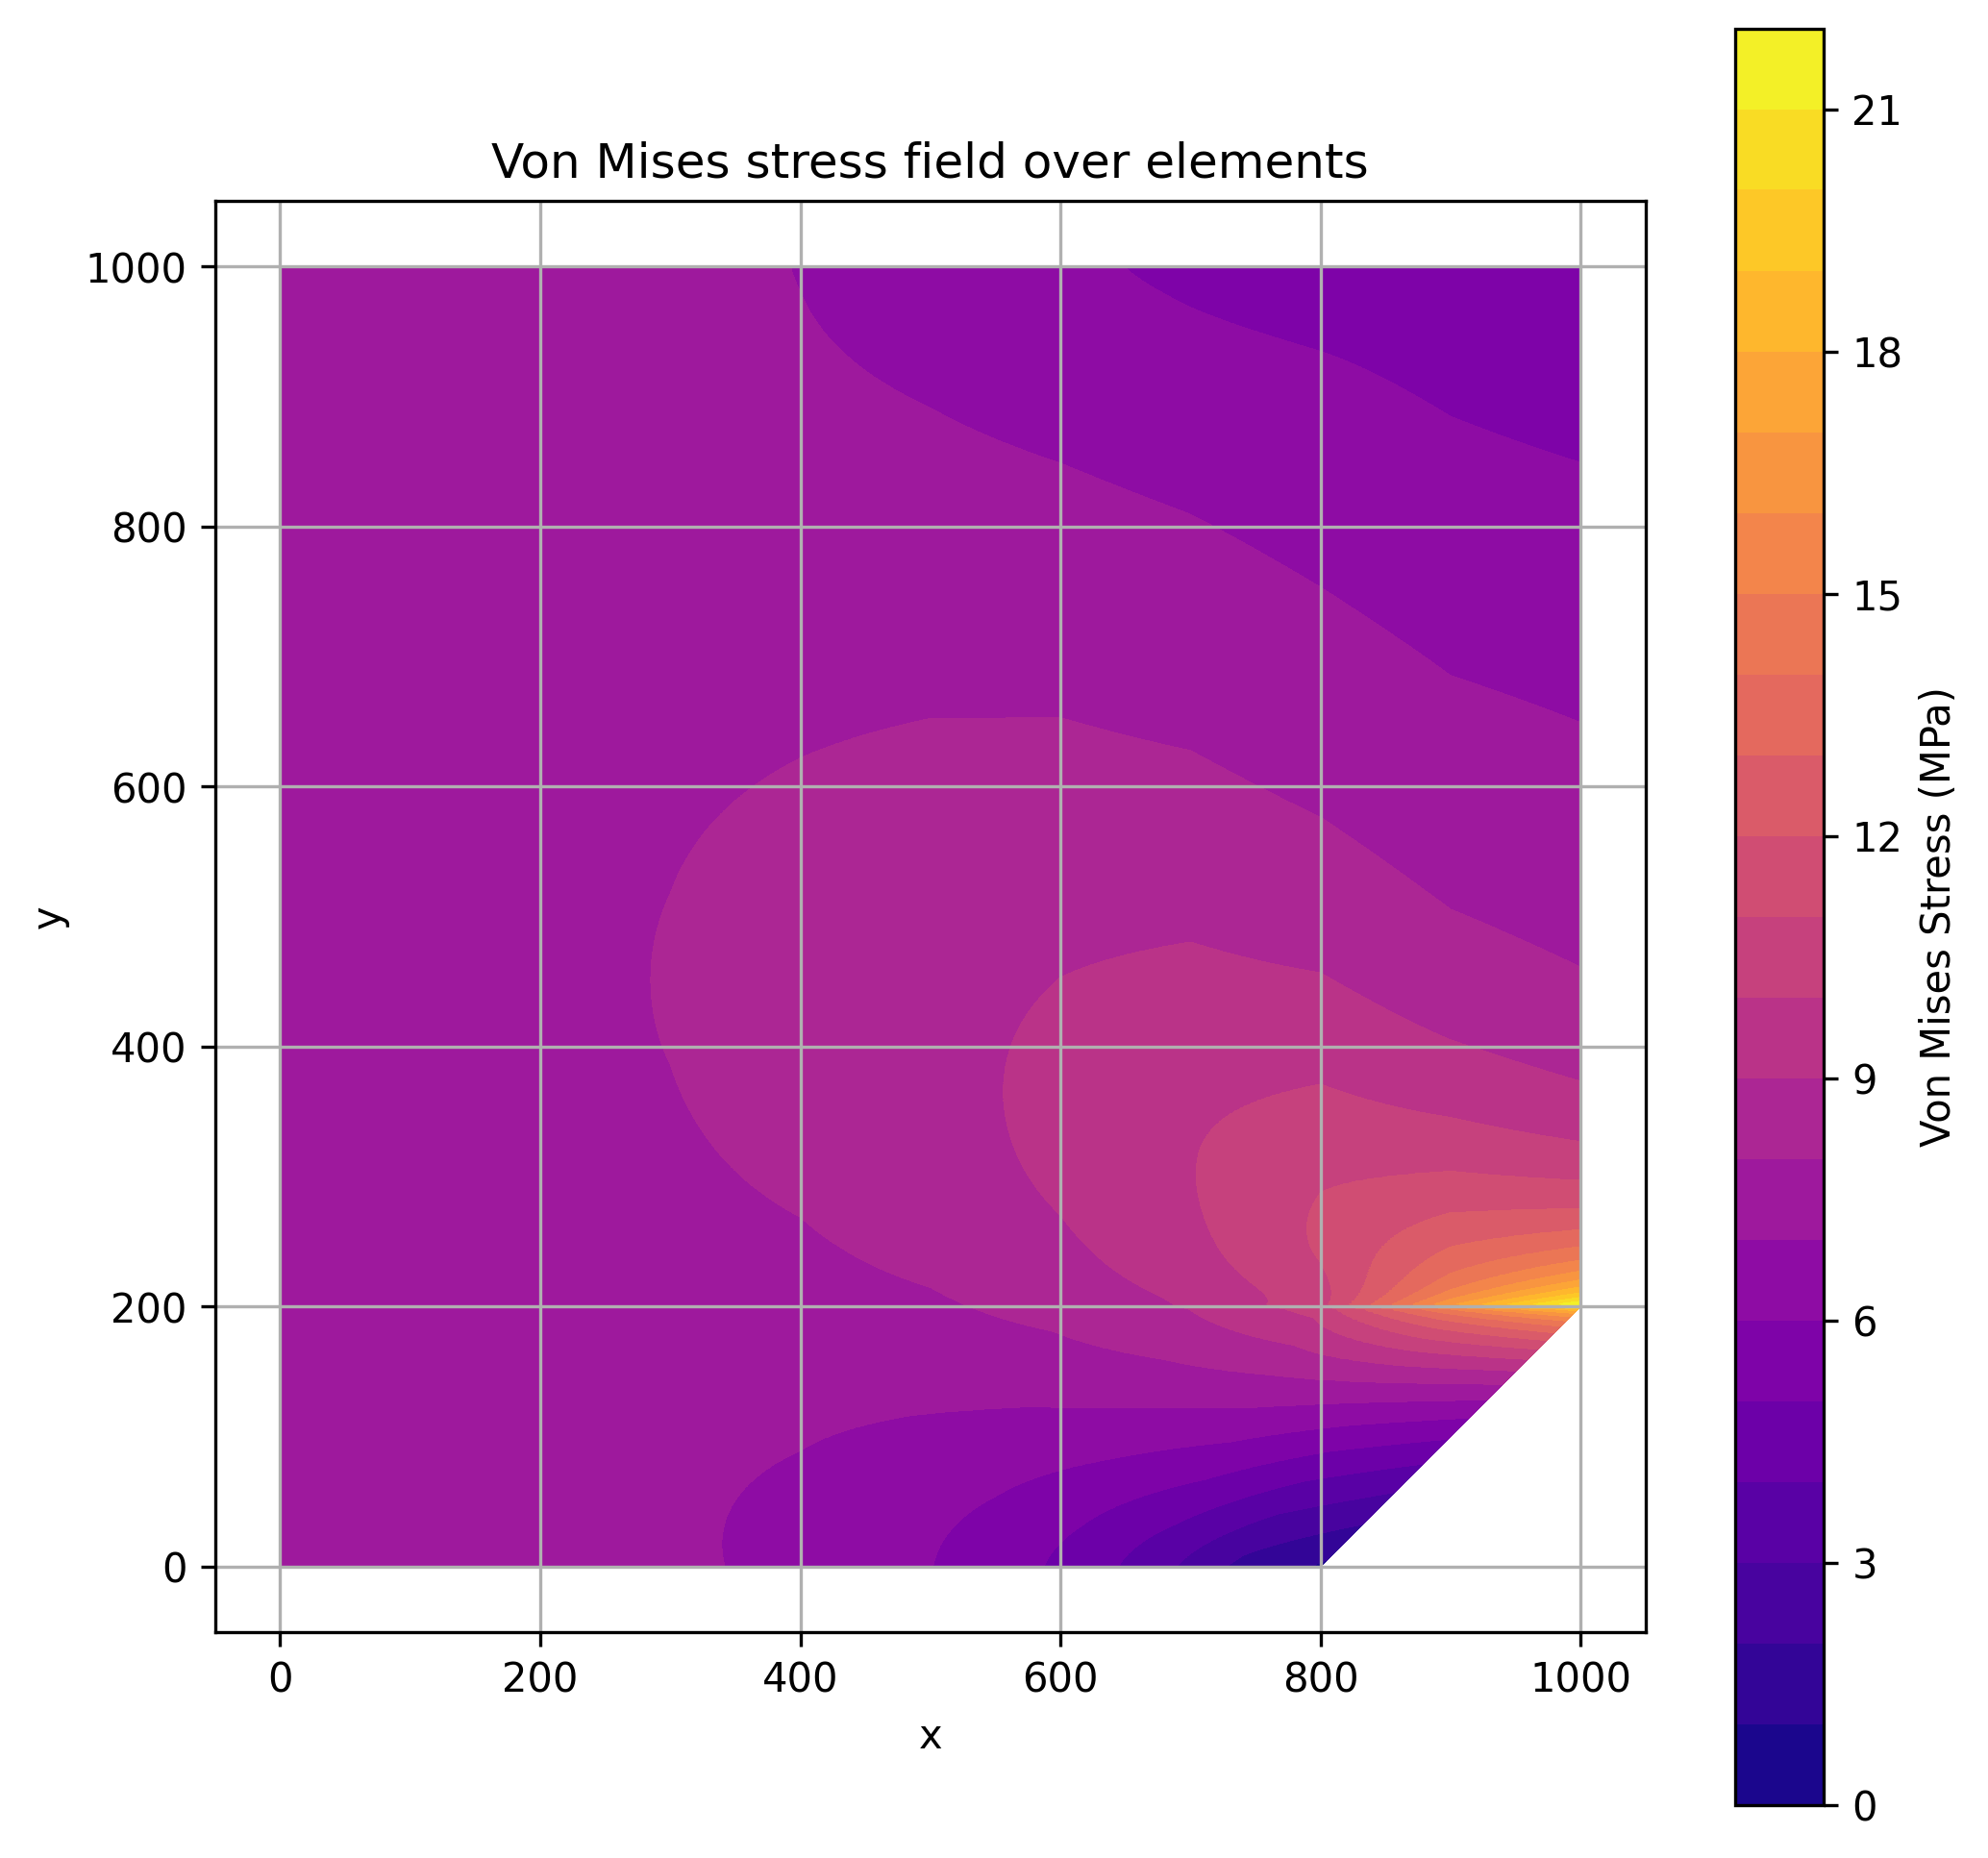
\includegraphics[width=\textwidth]{GRAFICOS/Quad9/2mm_global/resultados_von_mises.png}
    \caption{Global mesh refinement - $h=2mm$}
    \label{fig:img1}
  \end{subfigure}
  \hfill
  \begin{subfigure}[b]{0.45\textwidth}
    \centering
    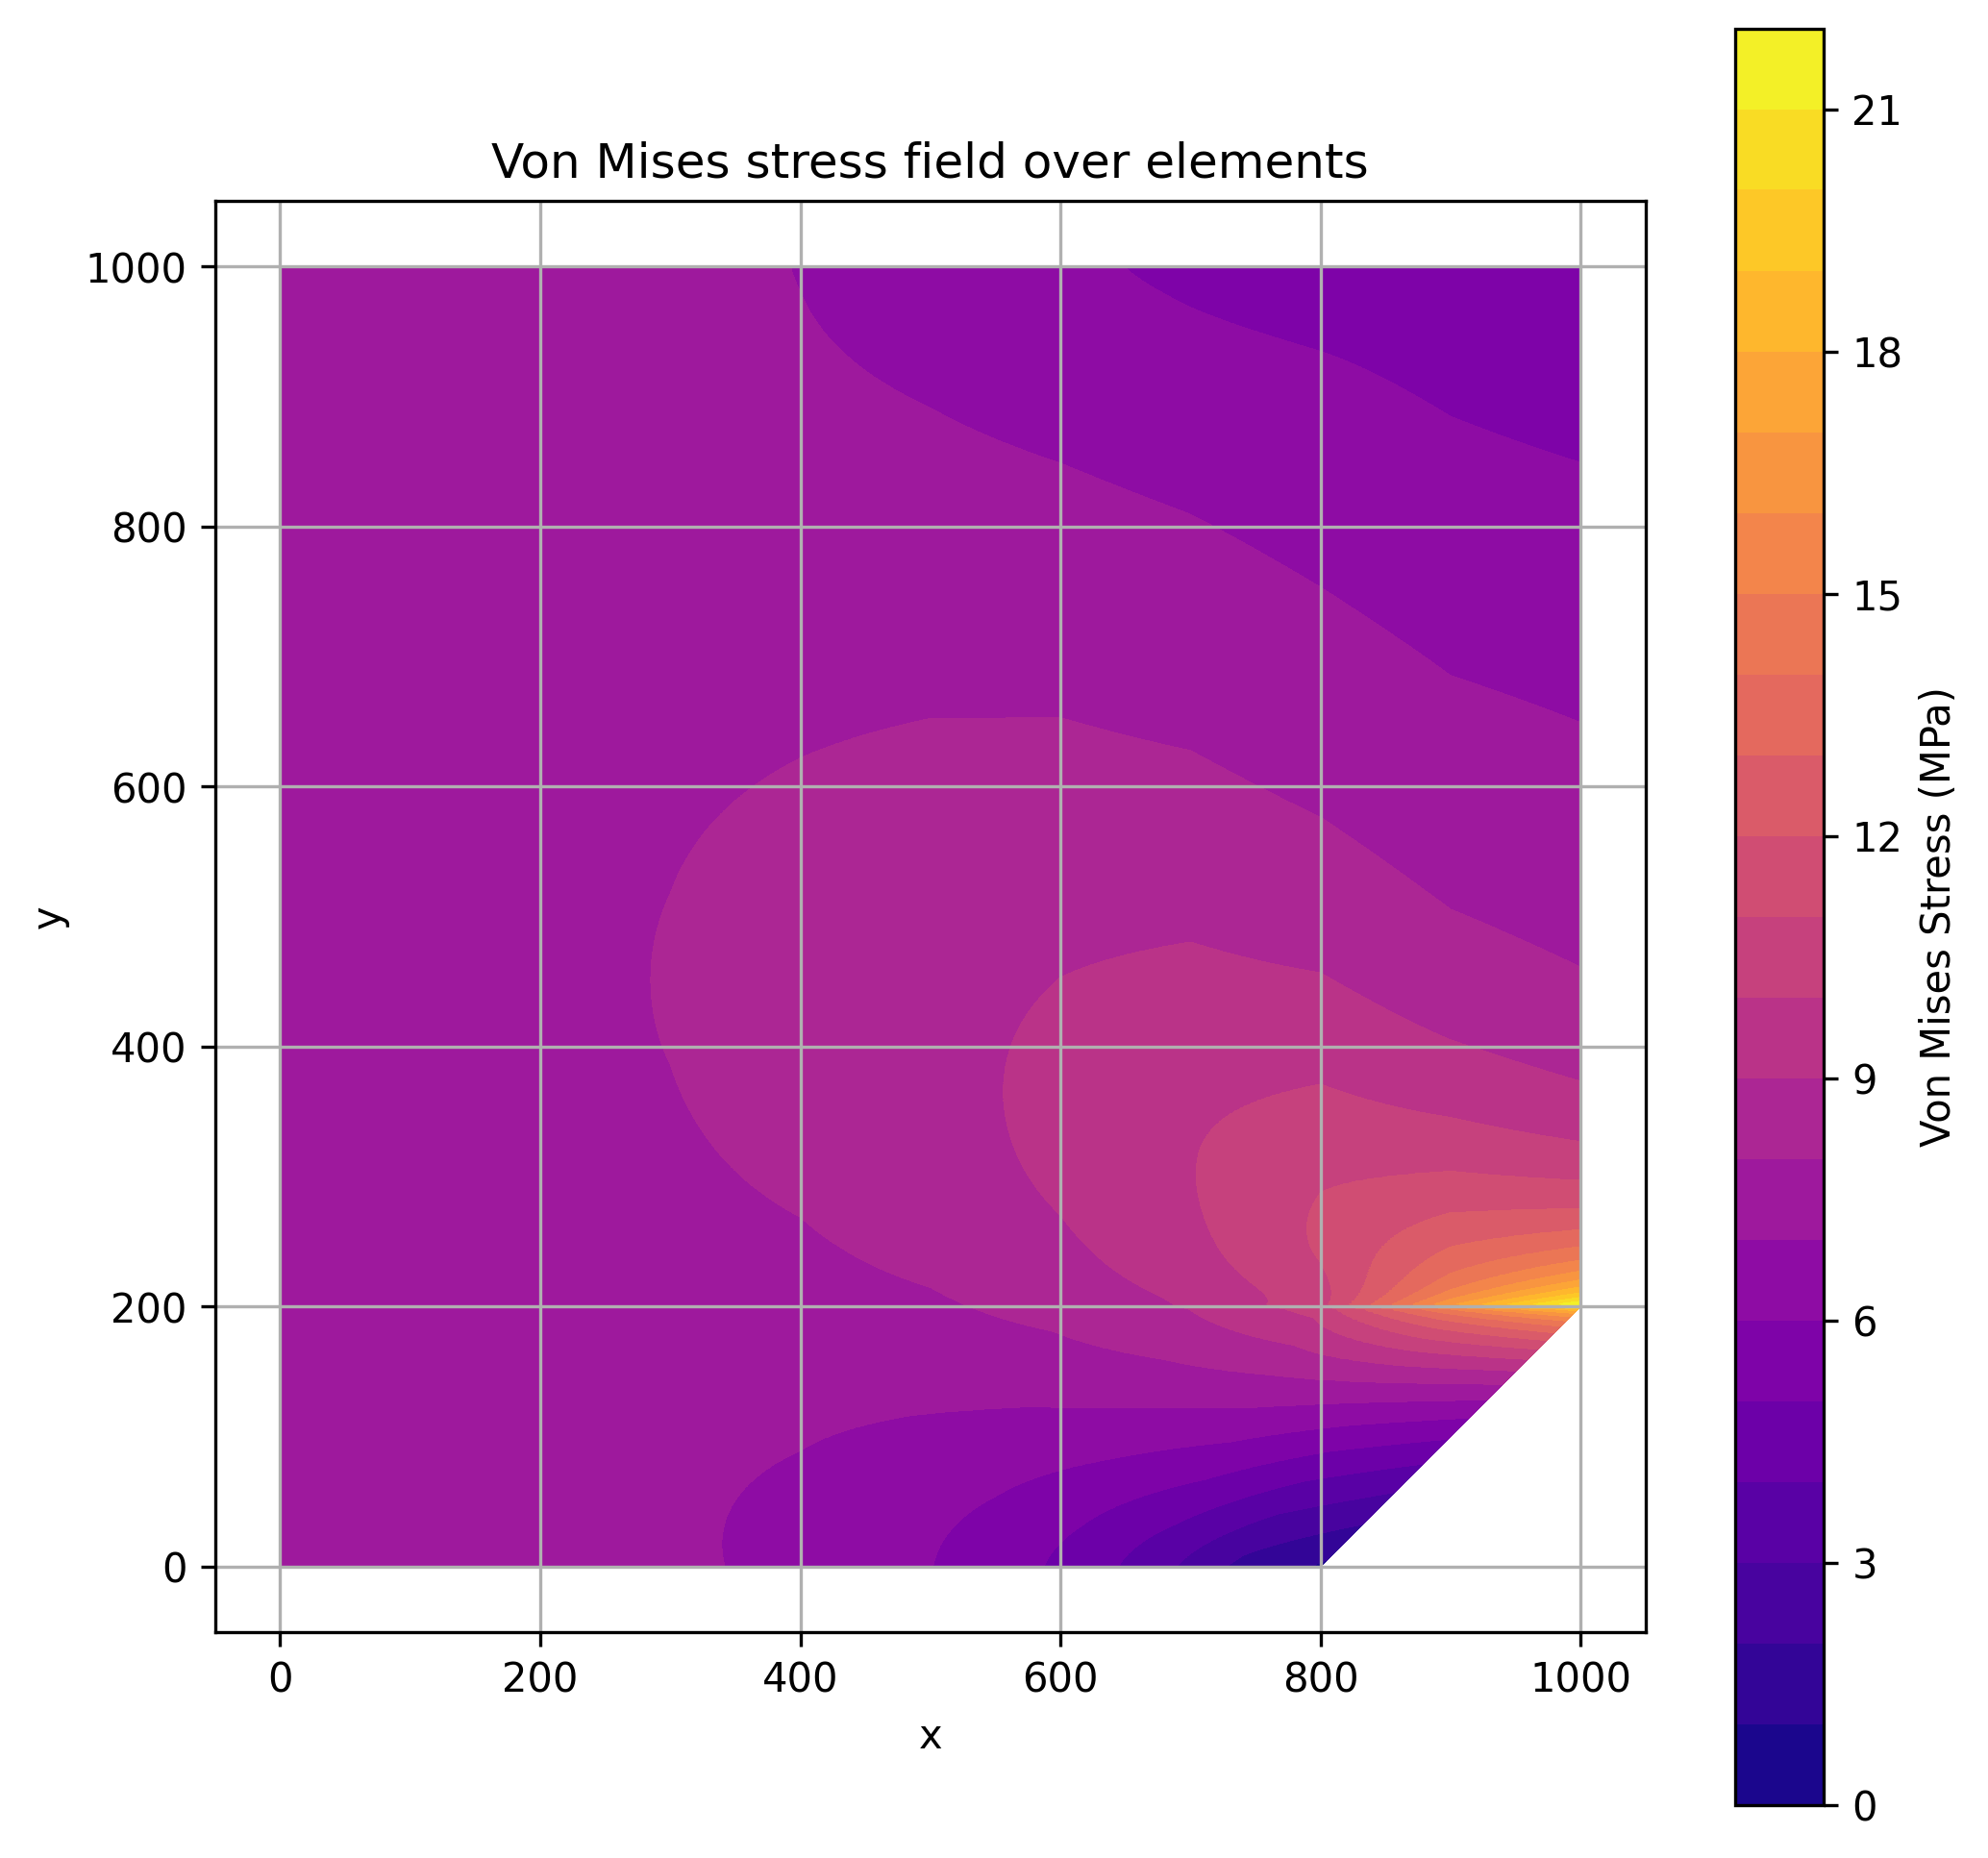
\includegraphics[width=\textwidth]{GRAFICOS/Quad9/2mm_global/resultados_von_mises.png}
    \caption{Local mesh refinement - $h=2mm$}
    \label{fig:img2}
  \end{subfigure}
\end{figure}

\begin{figure}[H]
  \centering
  \begin{subfigure}[b]{0.45\textwidth}
    \centering
    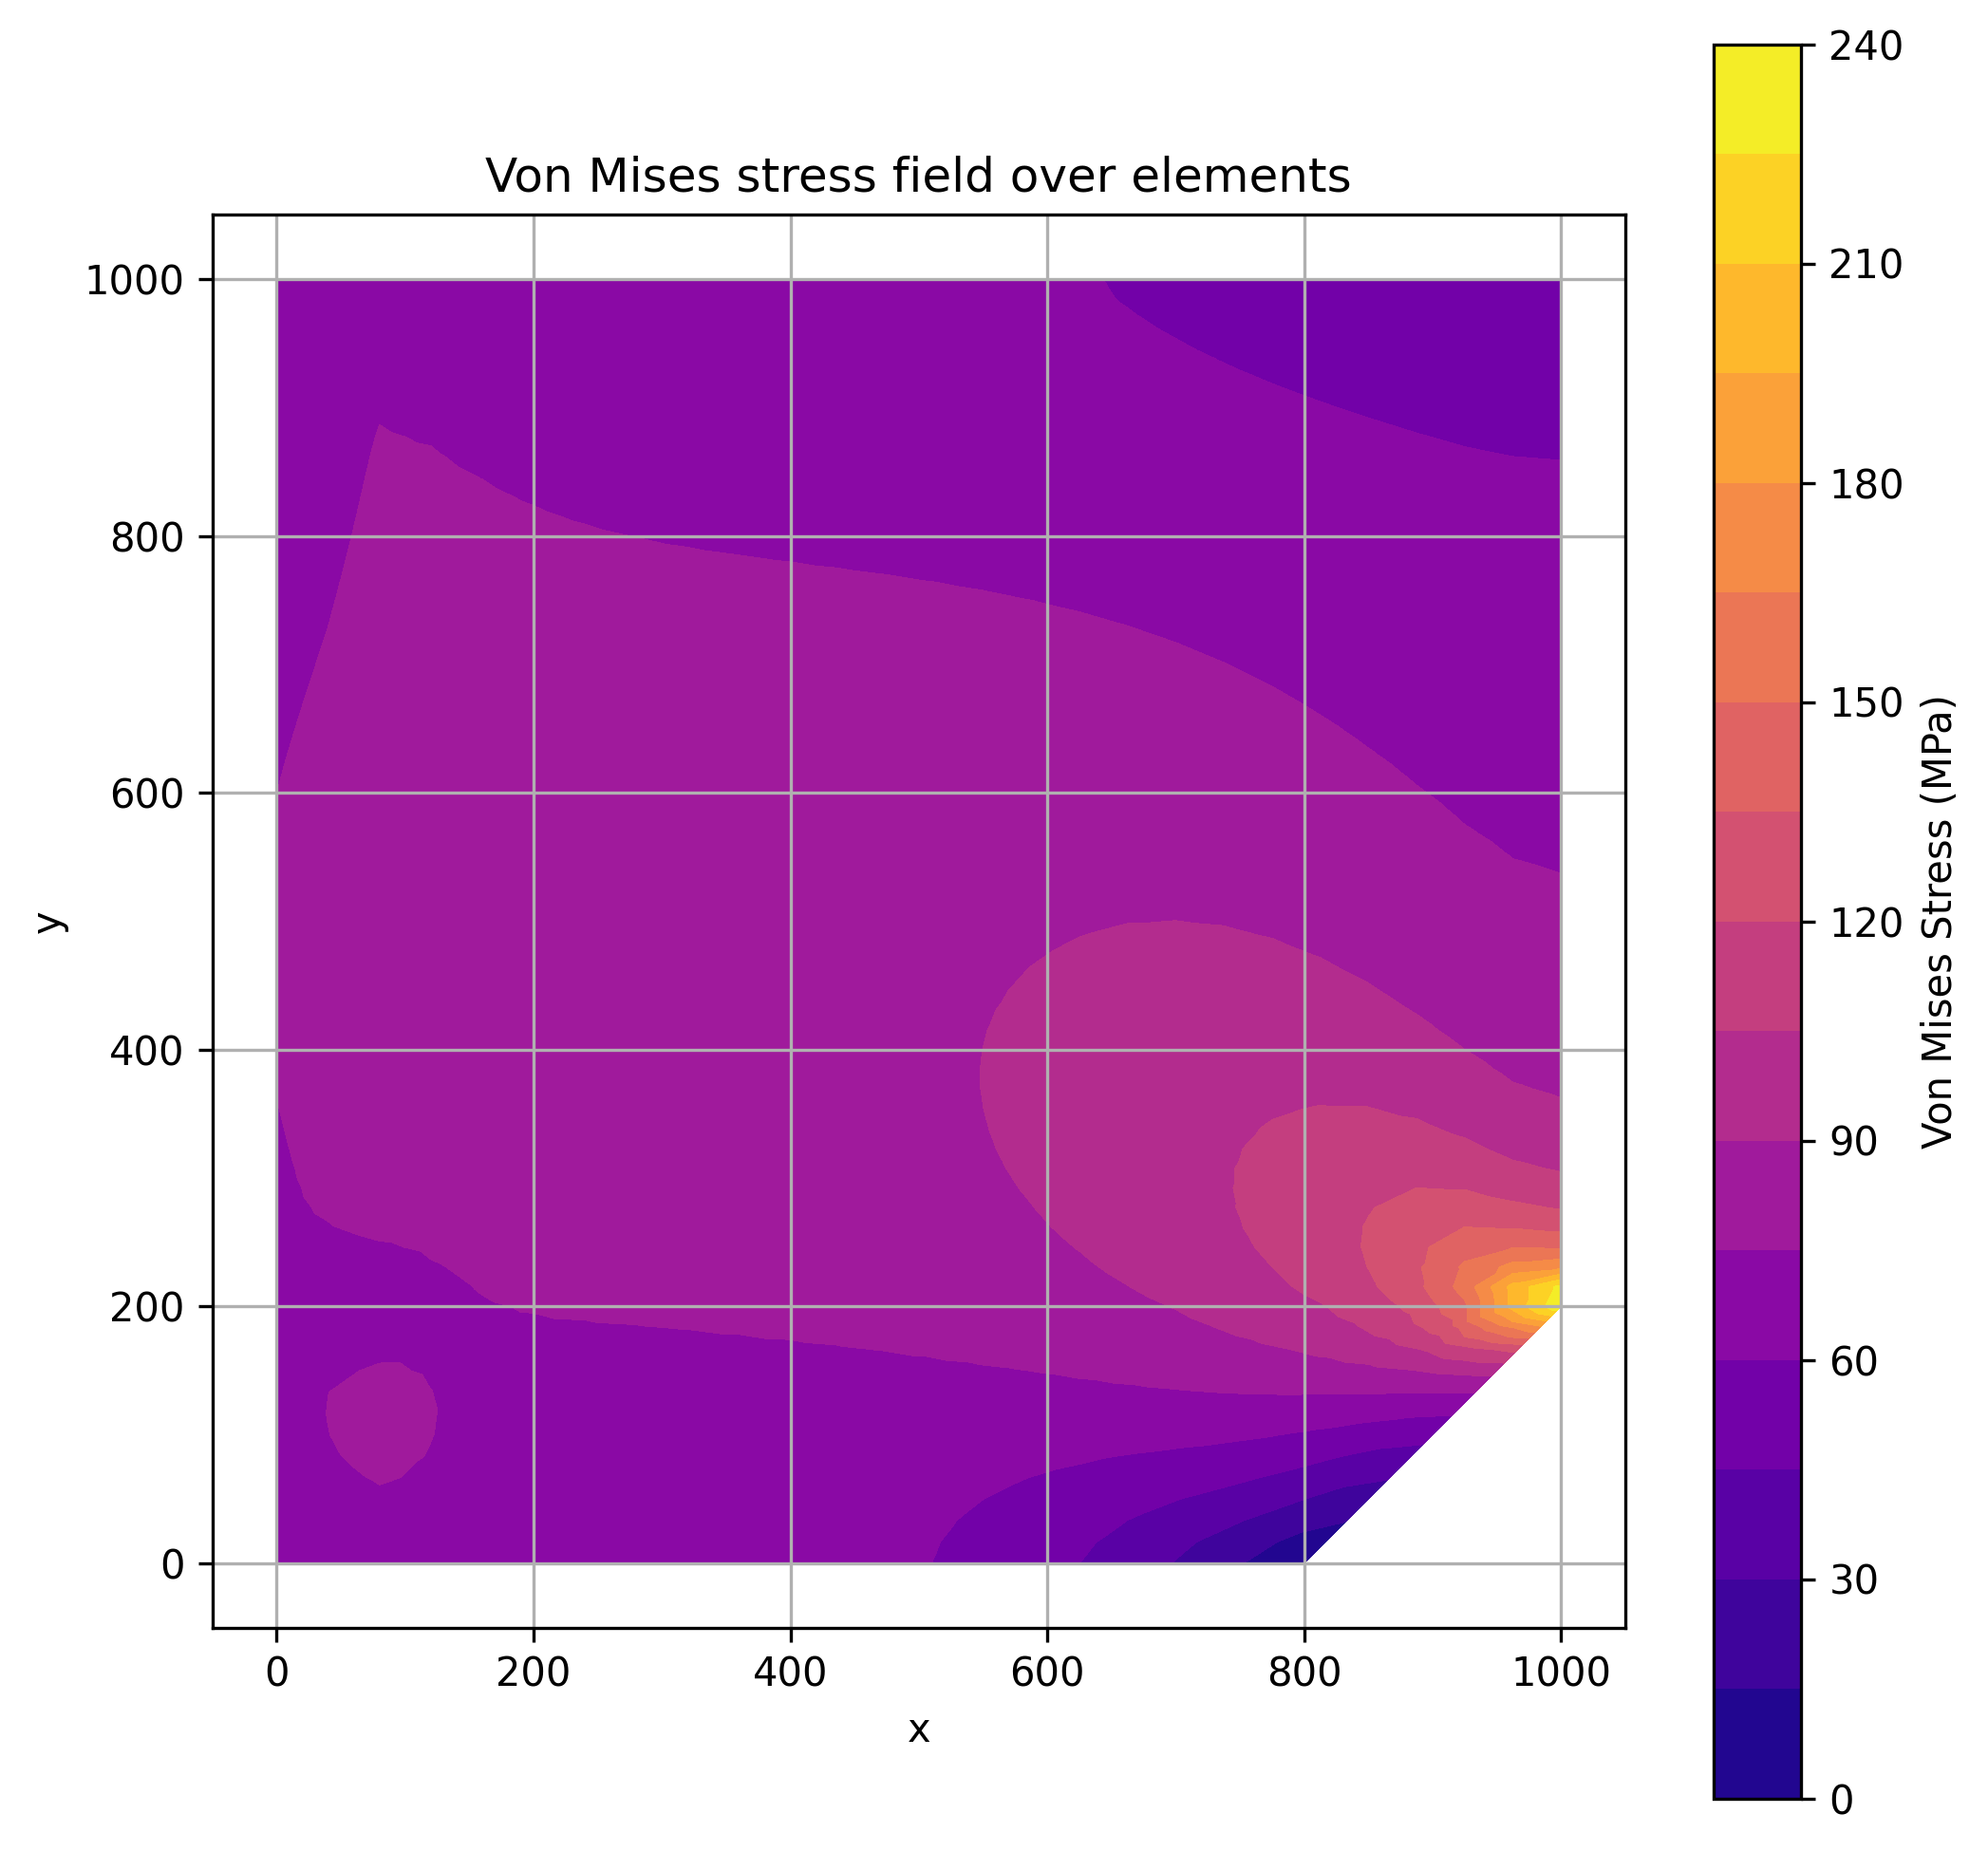
\includegraphics[width=\textwidth]{GRAFICOS/Quad9/1.75mm_global/resultados_von_mises.png}
    \caption{Global mesh refinement - $h=1.75mm$}
    \label{fig:img11}
  \end{subfigure}
  \hfill
  \begin{subfigure}[b]{0.45\textwidth}
    \centering
    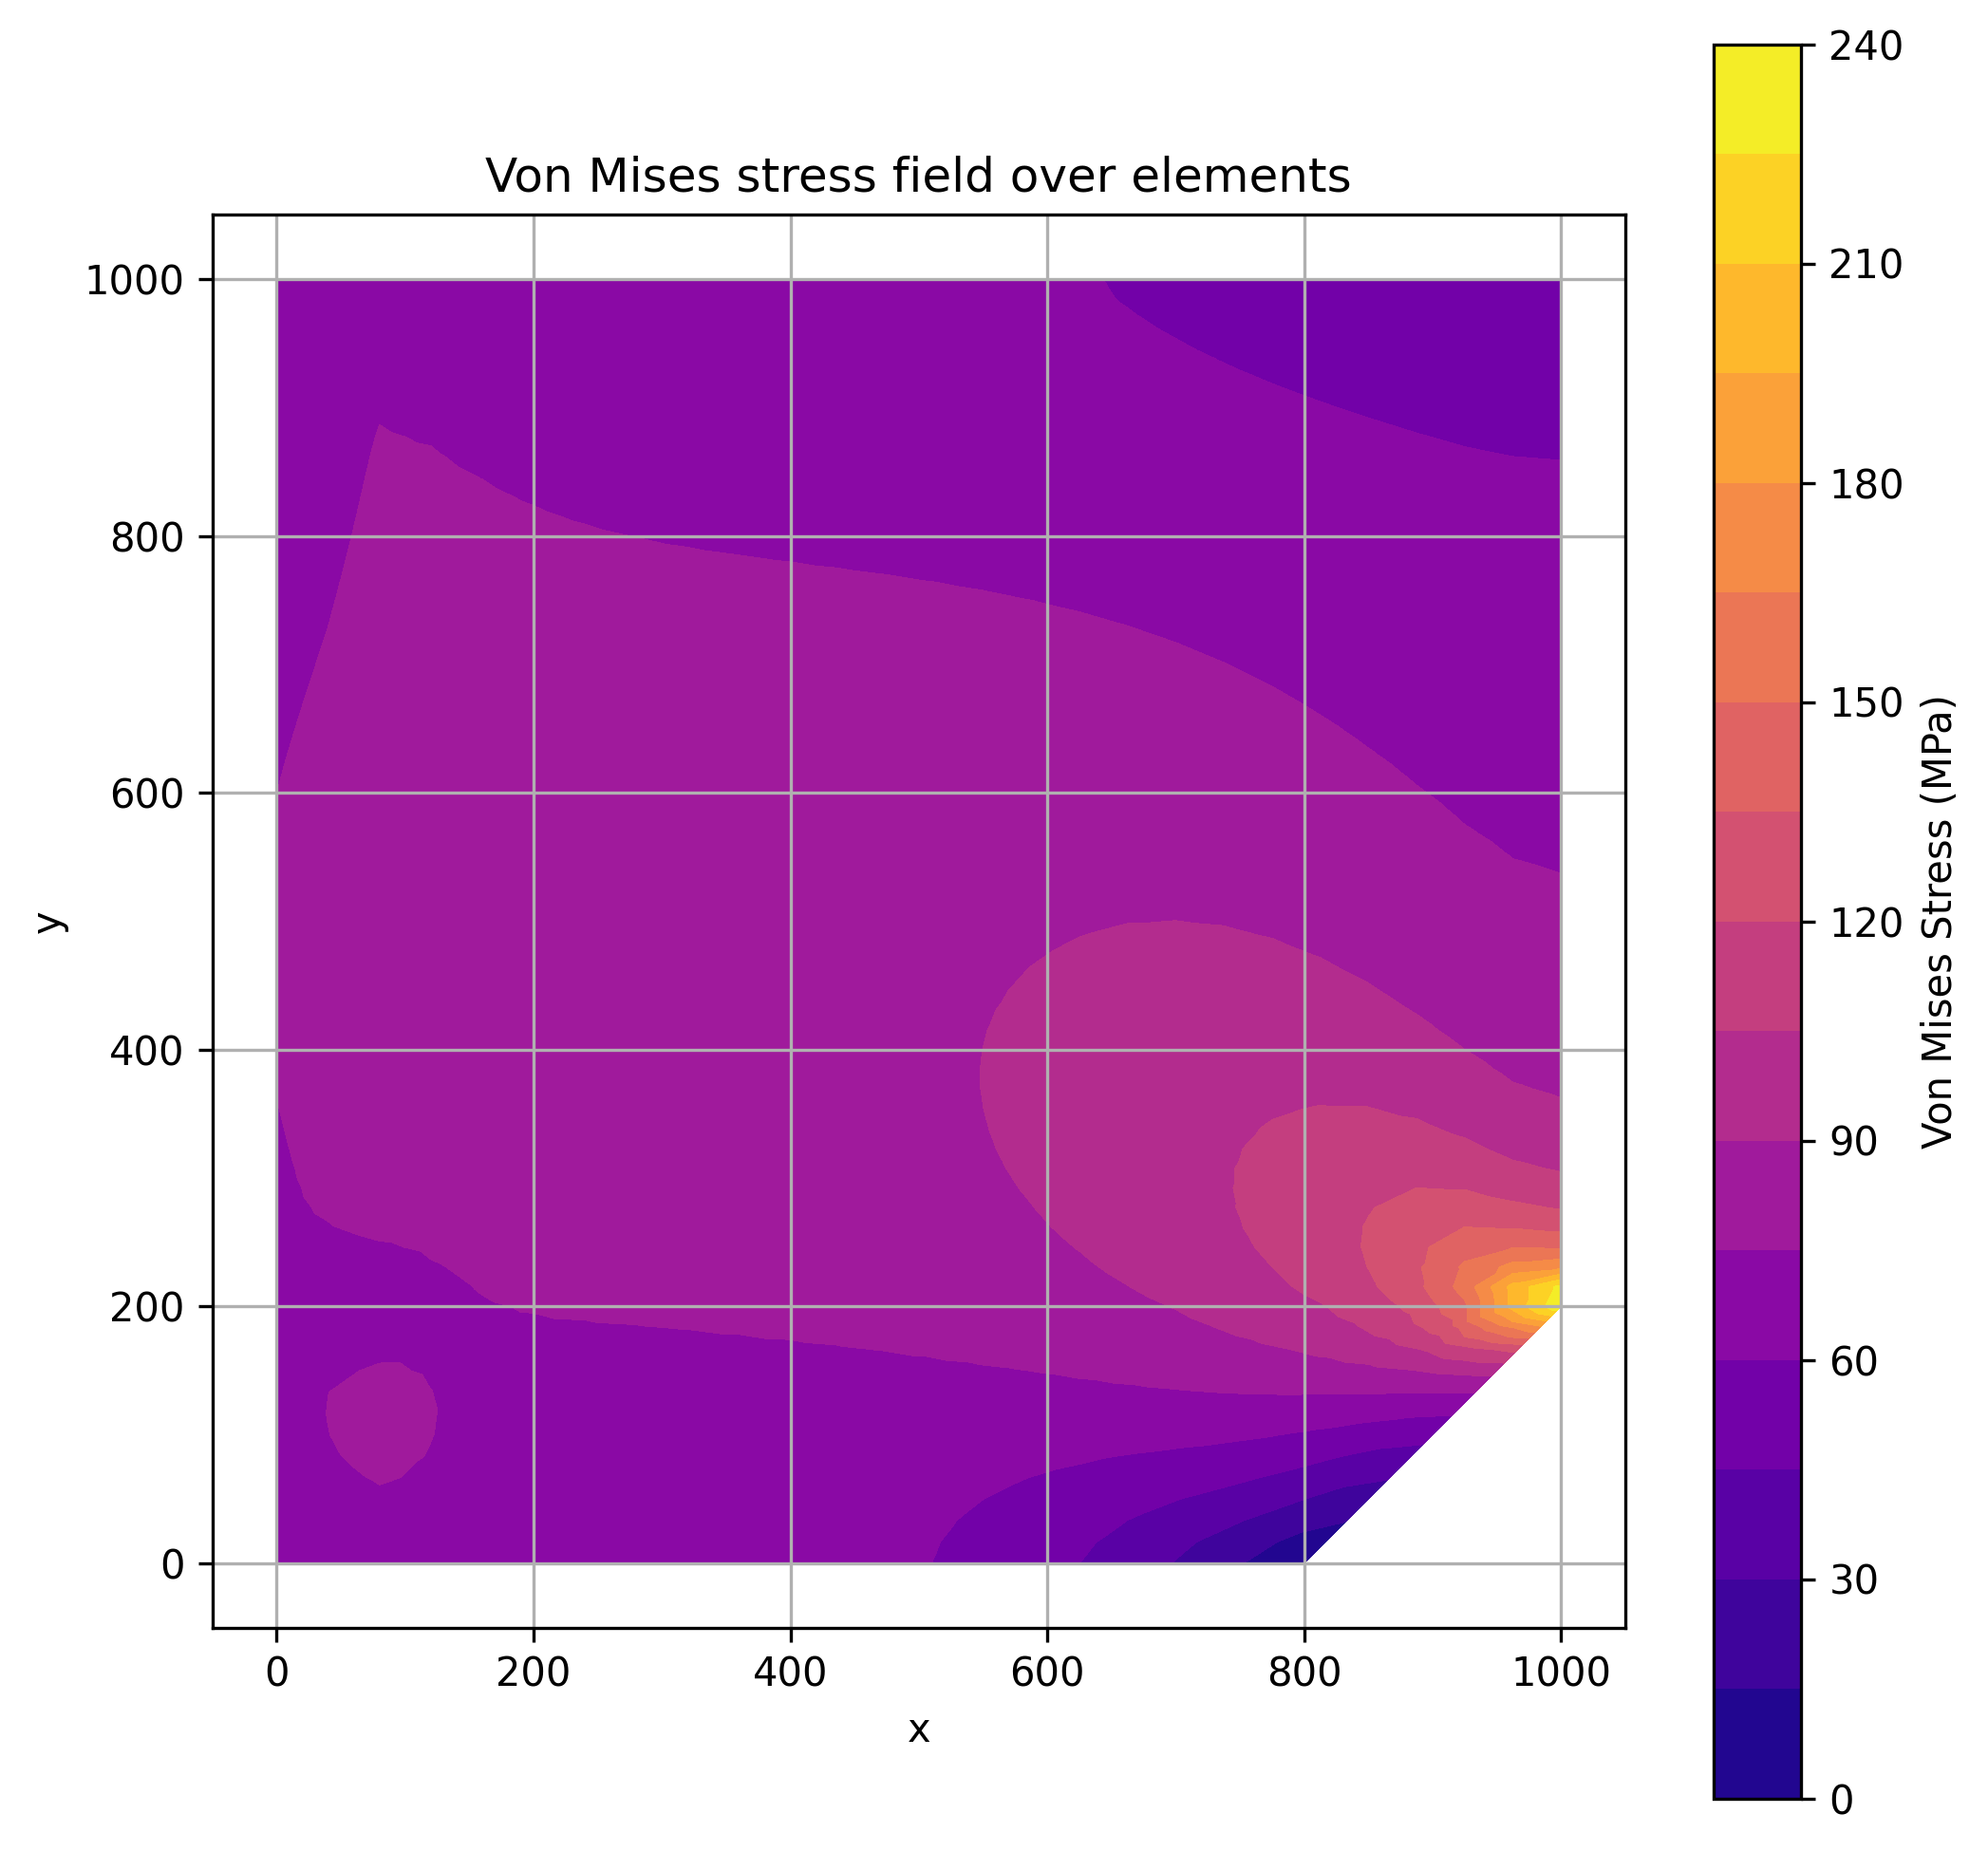
\includegraphics[width=\textwidth]{GRAFICOS/Quad9/1.75mm_global/resultados_von_mises.png}
    \caption{Local mesh refinement - $h=1.75mm$}
    \label{fig:img21}
  \end{subfigure}
\end{figure}

\begin{figure}[H]
  \centering
  \begin{subfigure}[b]{0.45\textwidth}
    \centering
    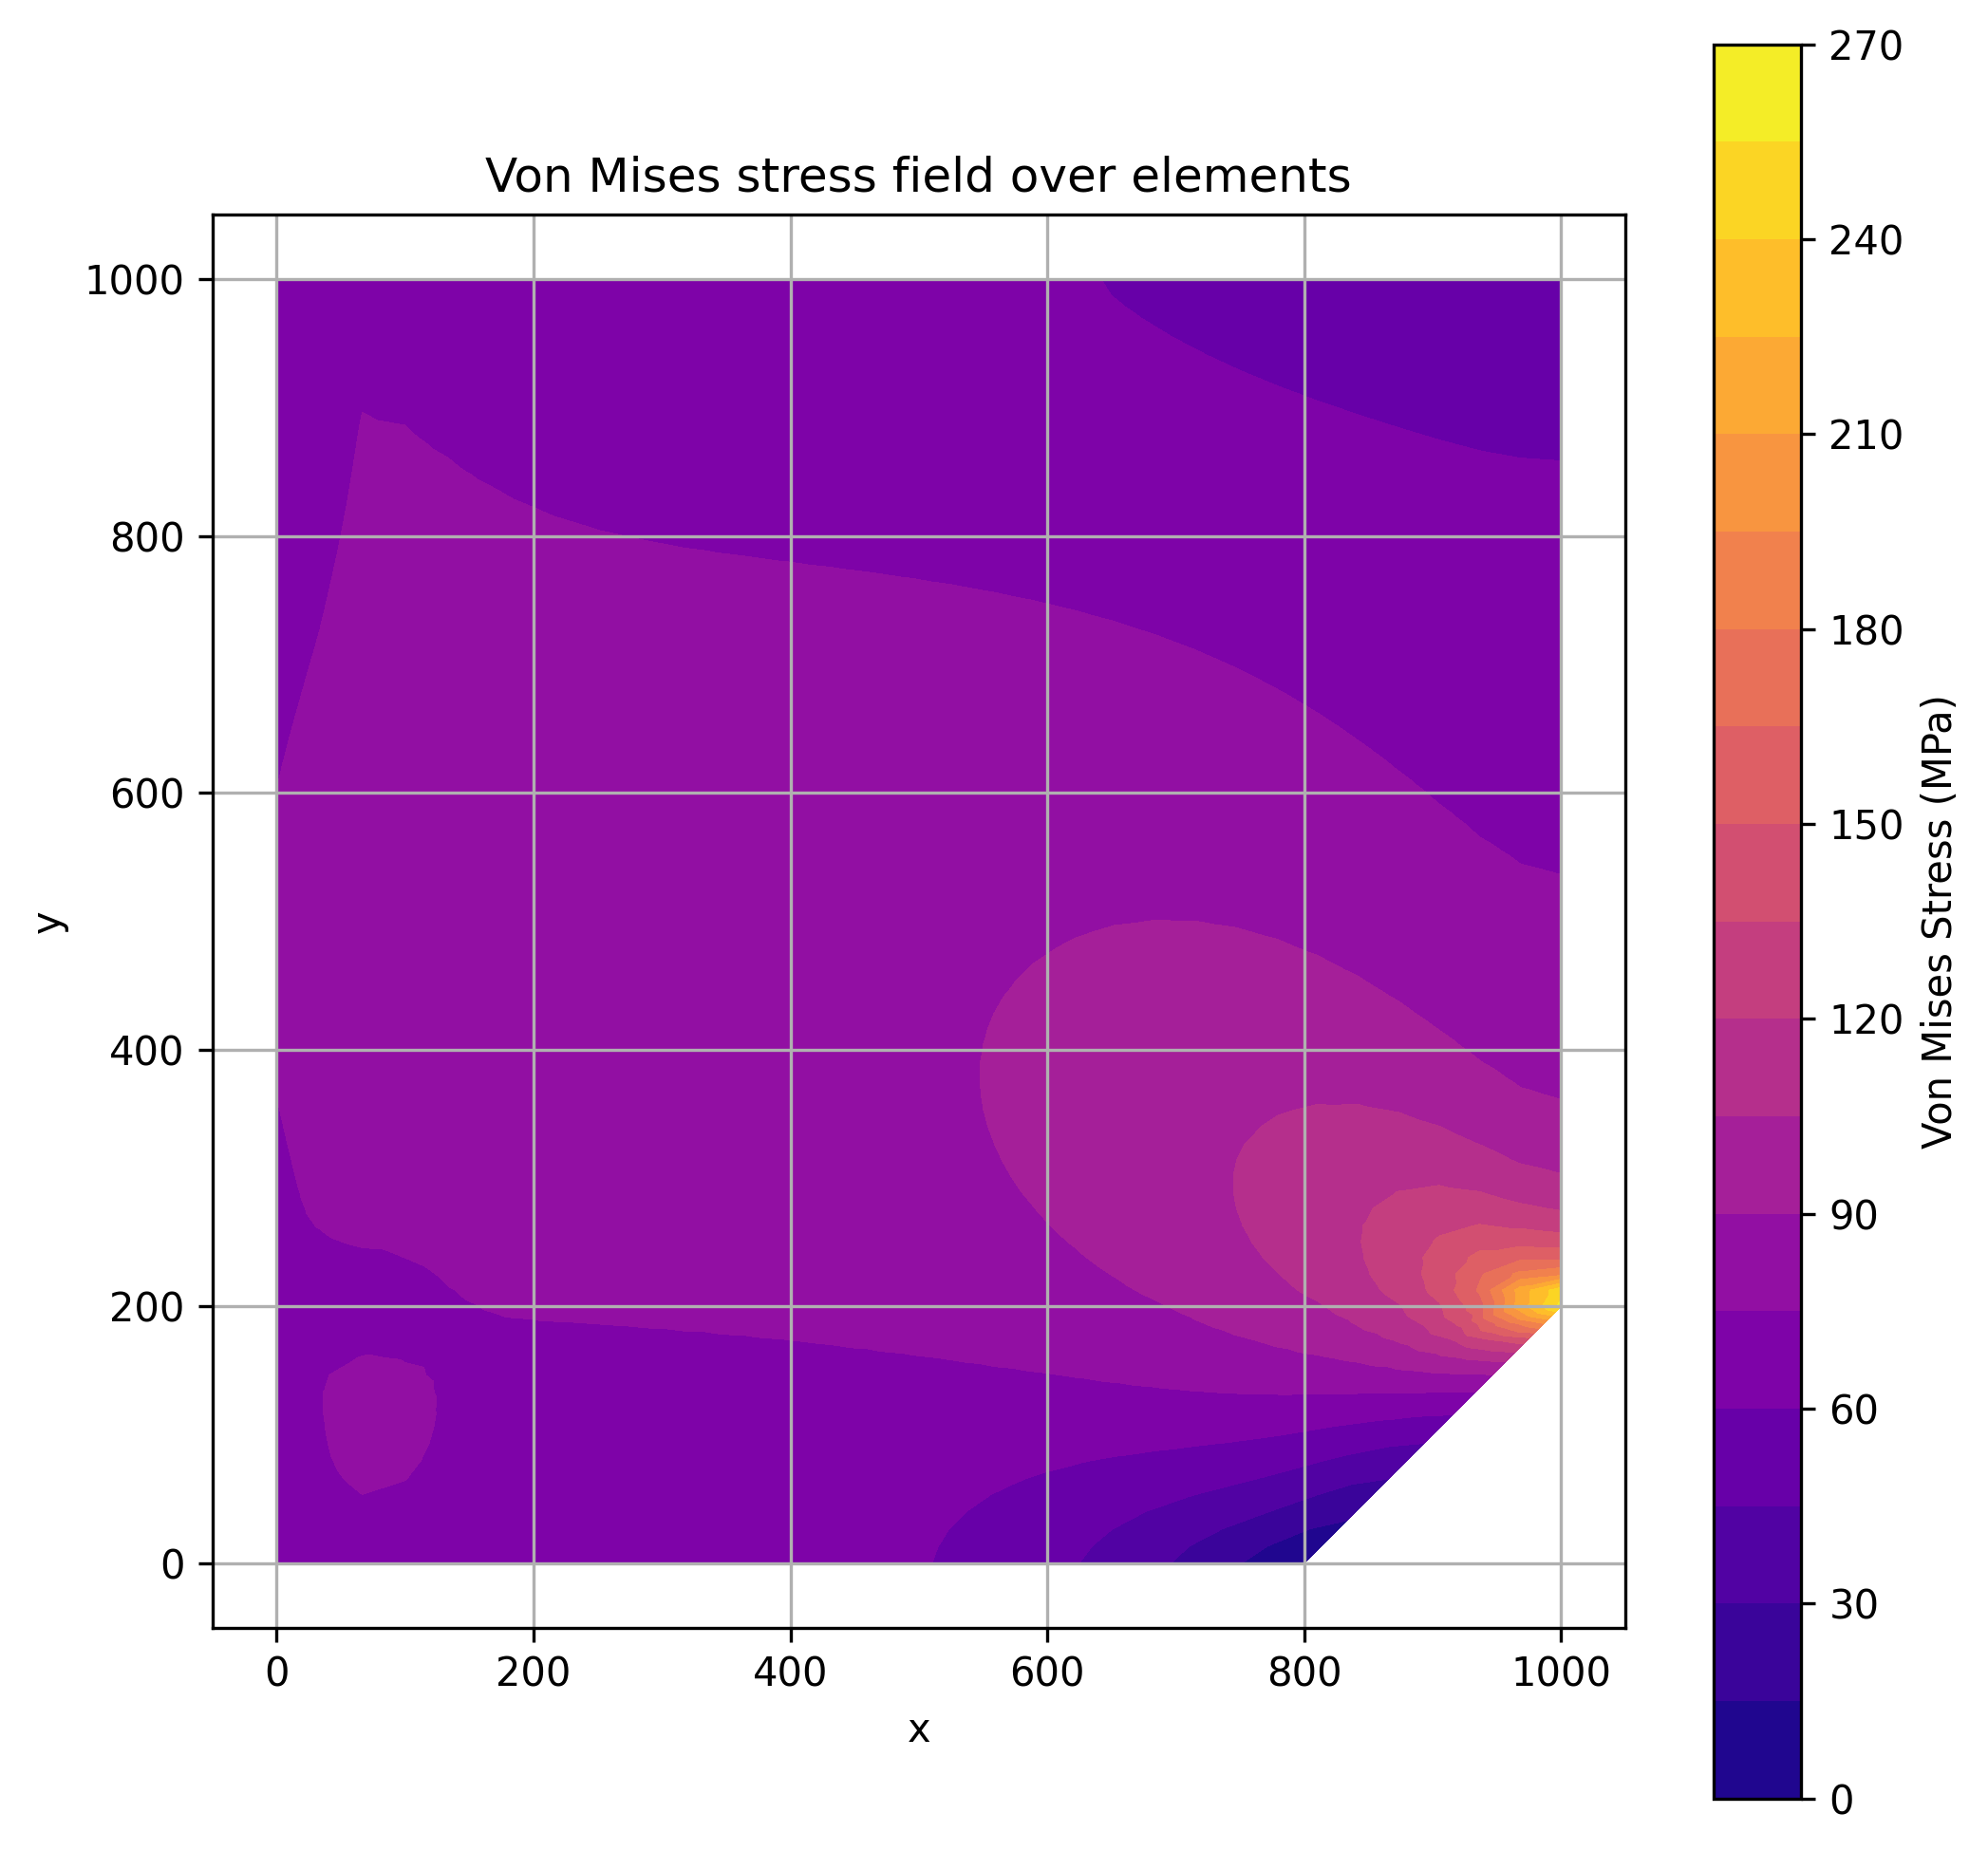
\includegraphics[width=\textwidth]{GRAFICOS/Quad9/1.5mm_global/resultados_von_mises.png}
    \caption{Global mesh refinement - $h=1.5mm$}
    \label{fig:img12}
  \end{subfigure}
  \hfill
  \begin{subfigure}[b]{0.45\textwidth}
    \centering
    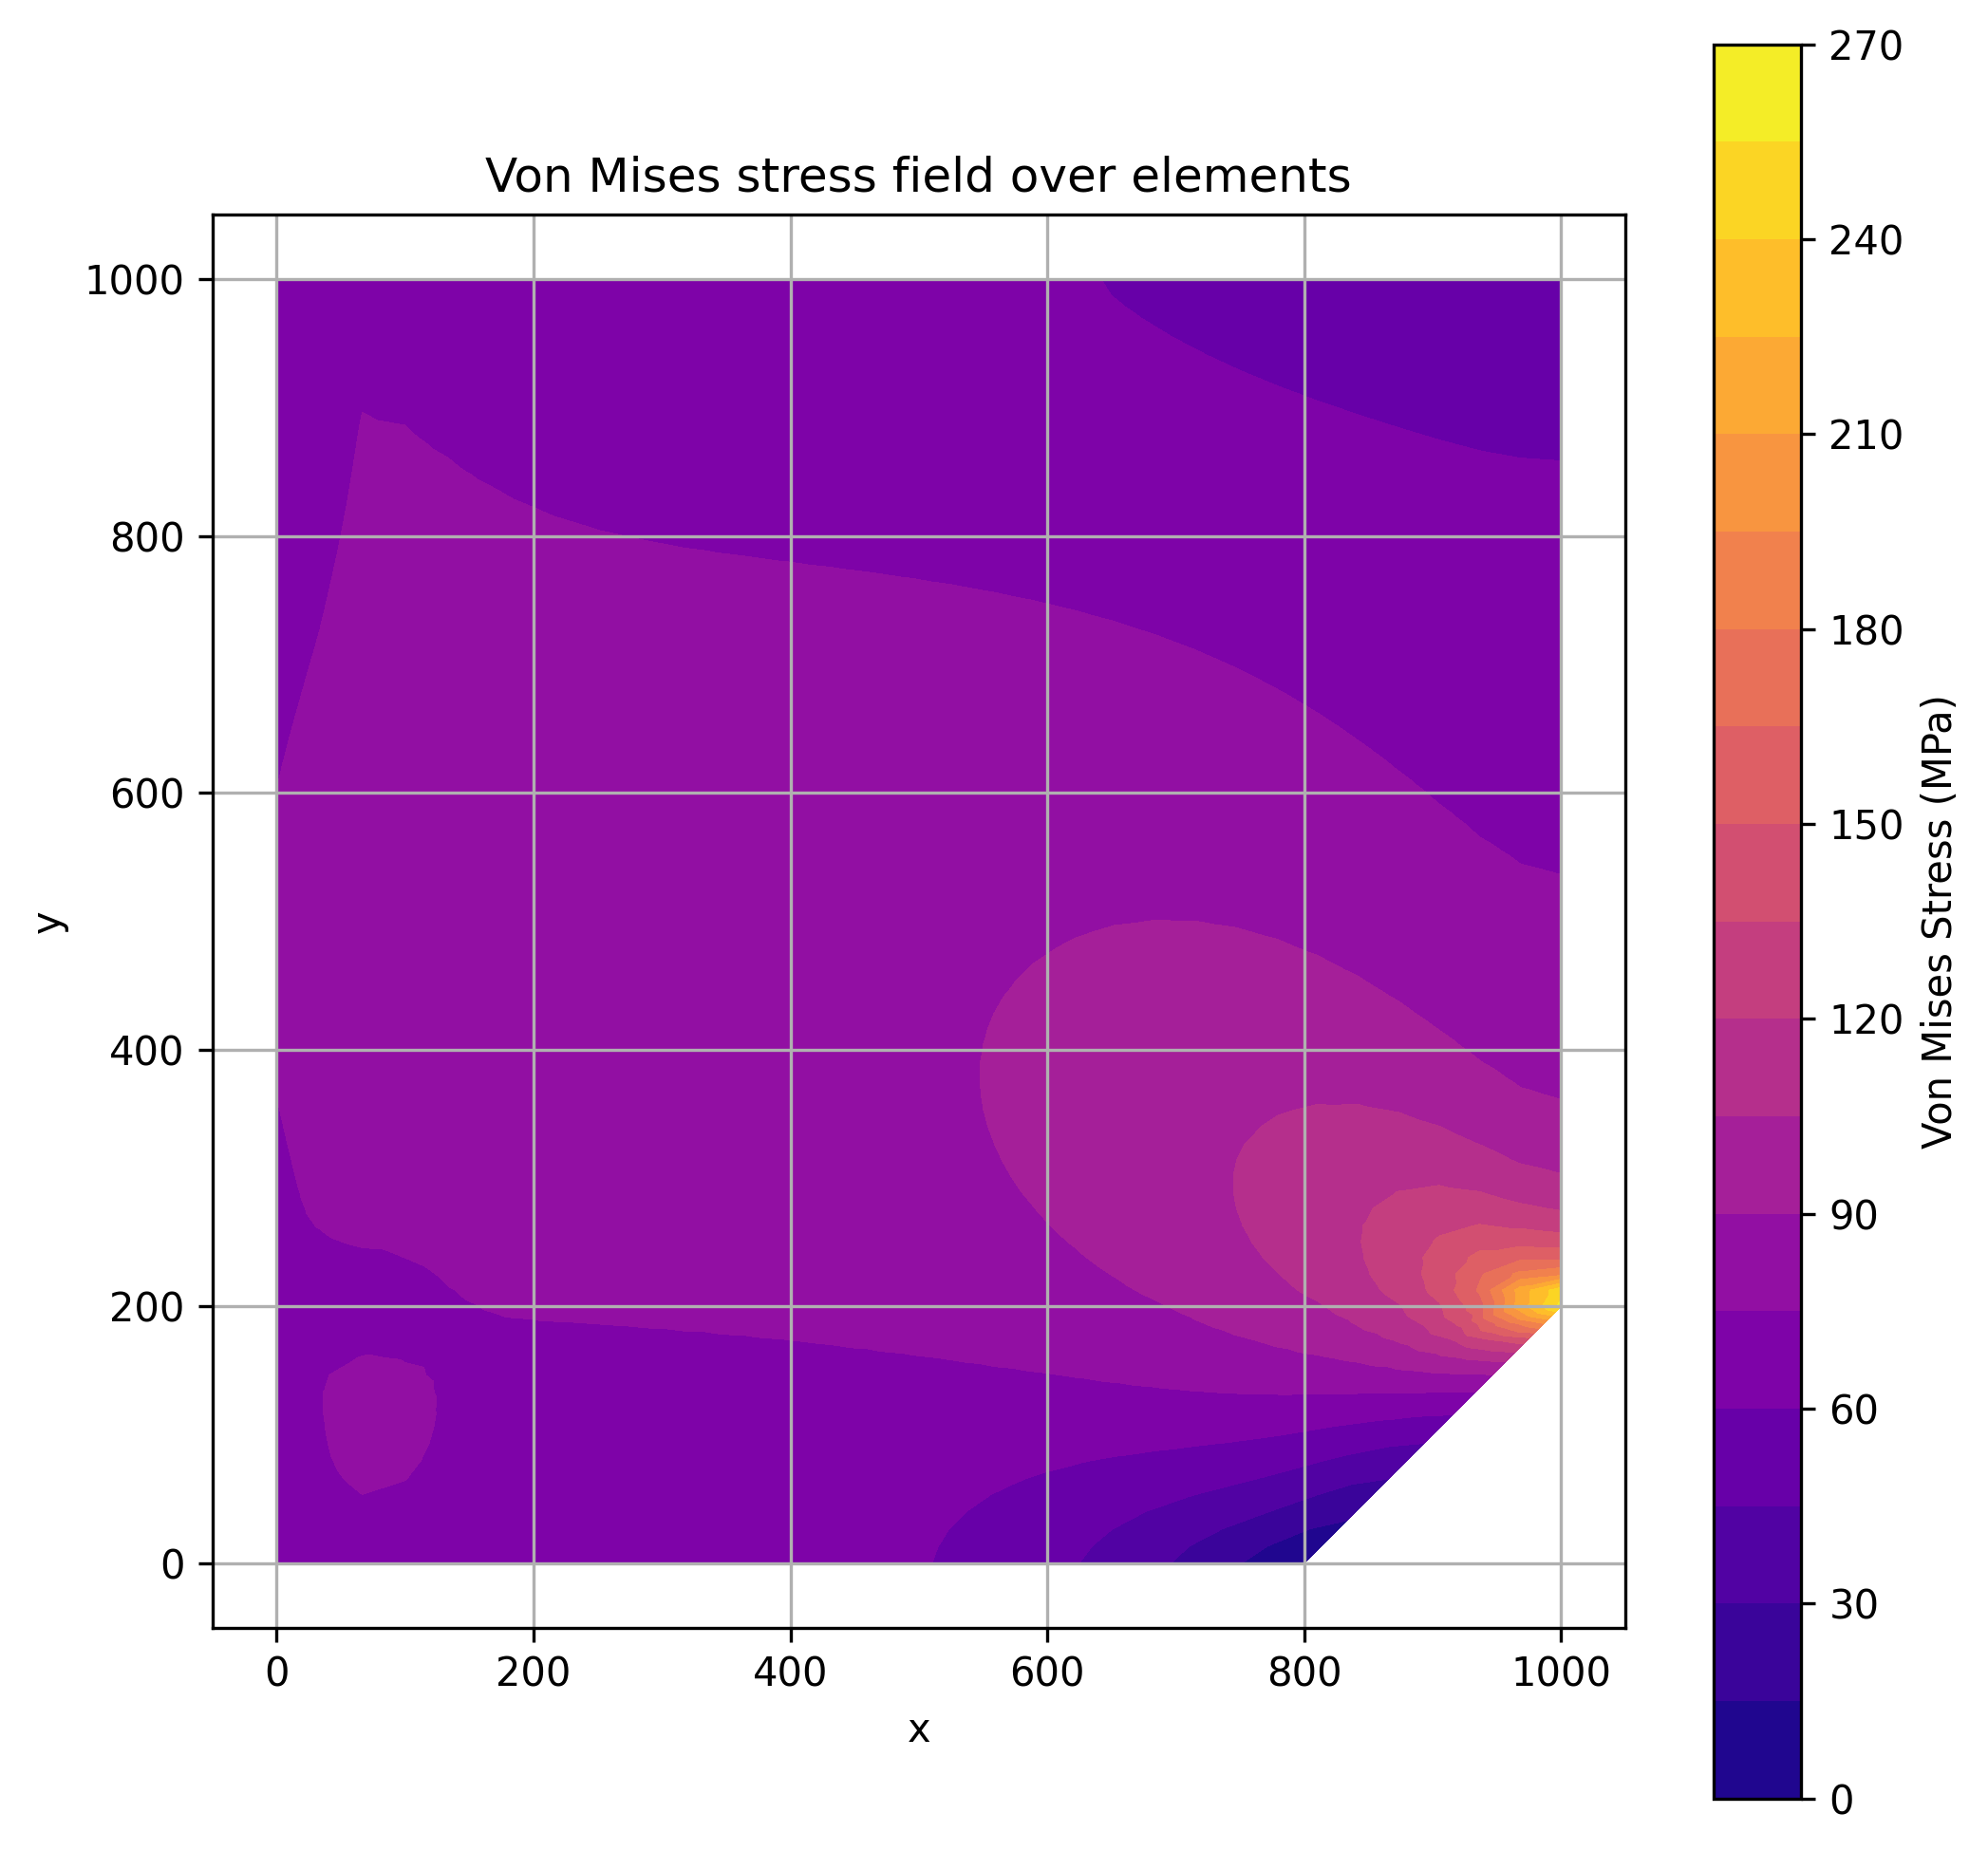
\includegraphics[width=\textwidth]{GRAFICOS/Quad9/1.5mm_global/resultados_von_mises.png}
    \caption{Local mesh refinement - $h=1.5mm$}
    \label{fig:img22}
  \end{subfigure}
\end{figure}

\begin{figure}[H]
  \centering
  \begin{subfigure}[b]{0.45\textwidth}
    \centering
    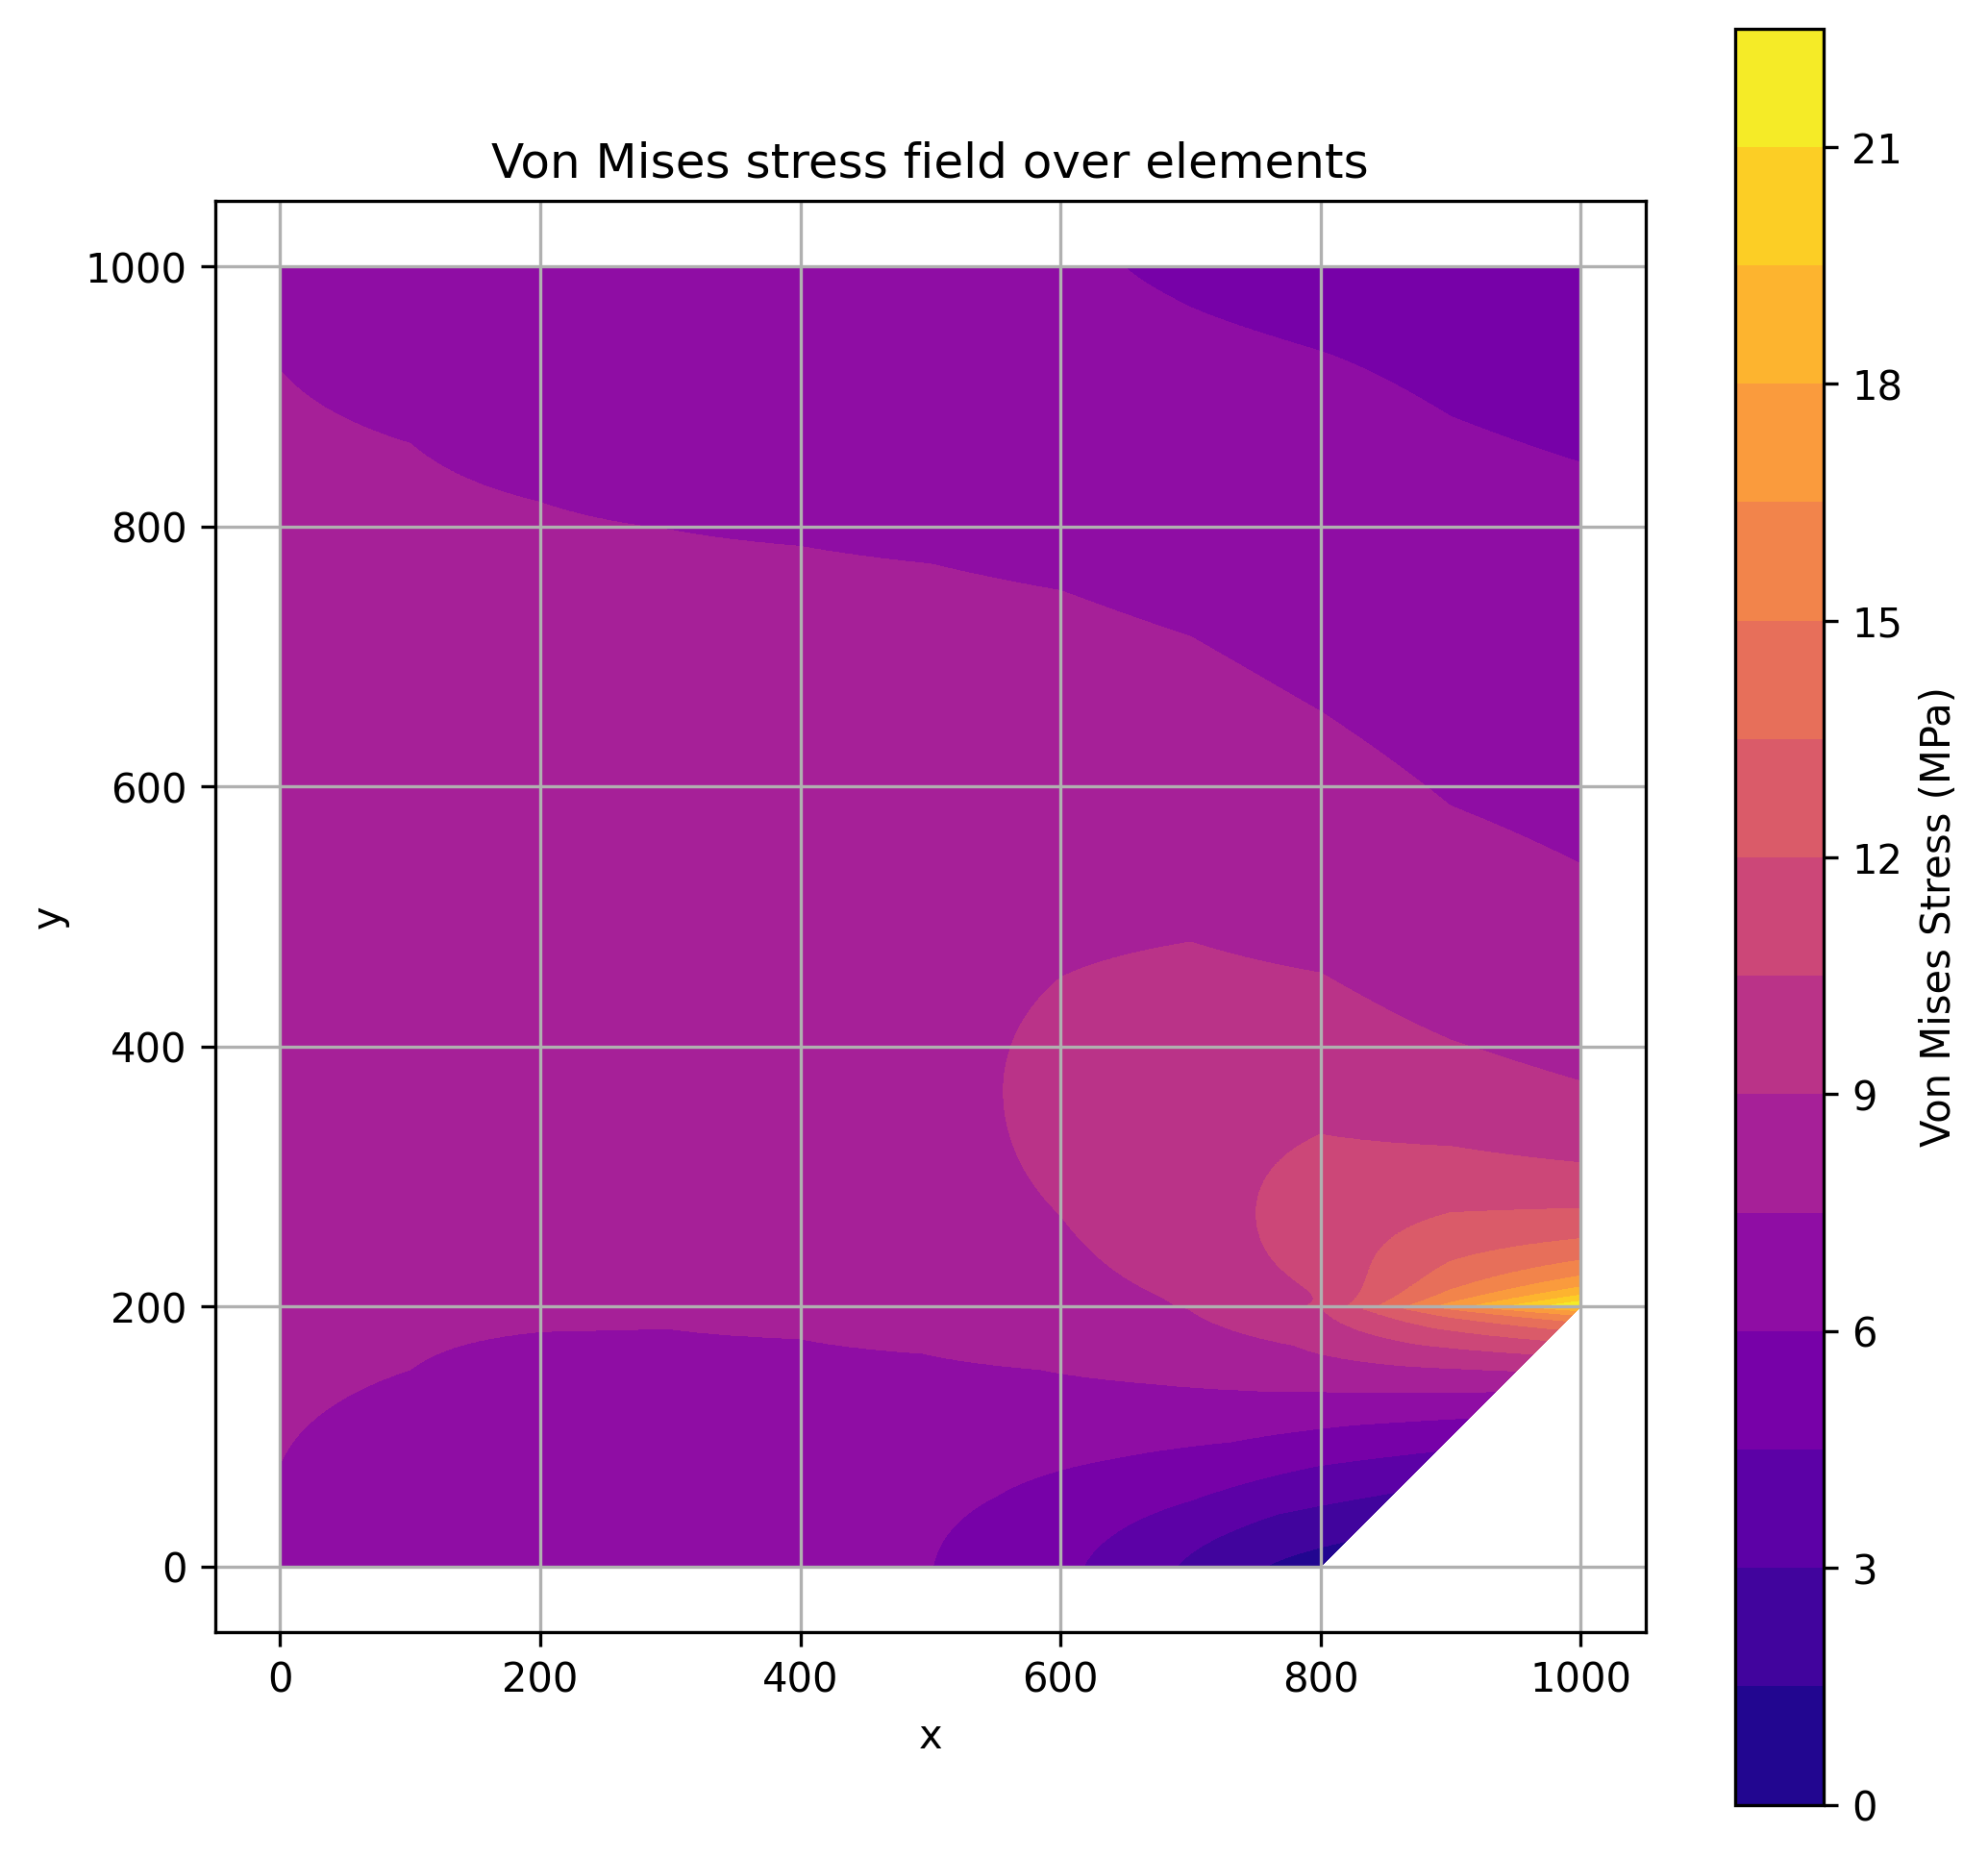
\includegraphics[width=\textwidth]{GRAFICOS/Quad9/1.25mm_global/resultados_von_mises.png}
    \caption{Global mesh refinement - $h=1.25mm$}
    \label{fig:img13}
  \end{subfigure}
  \hfill
  \begin{subfigure}[b]{0.45\textwidth}
    \centering
    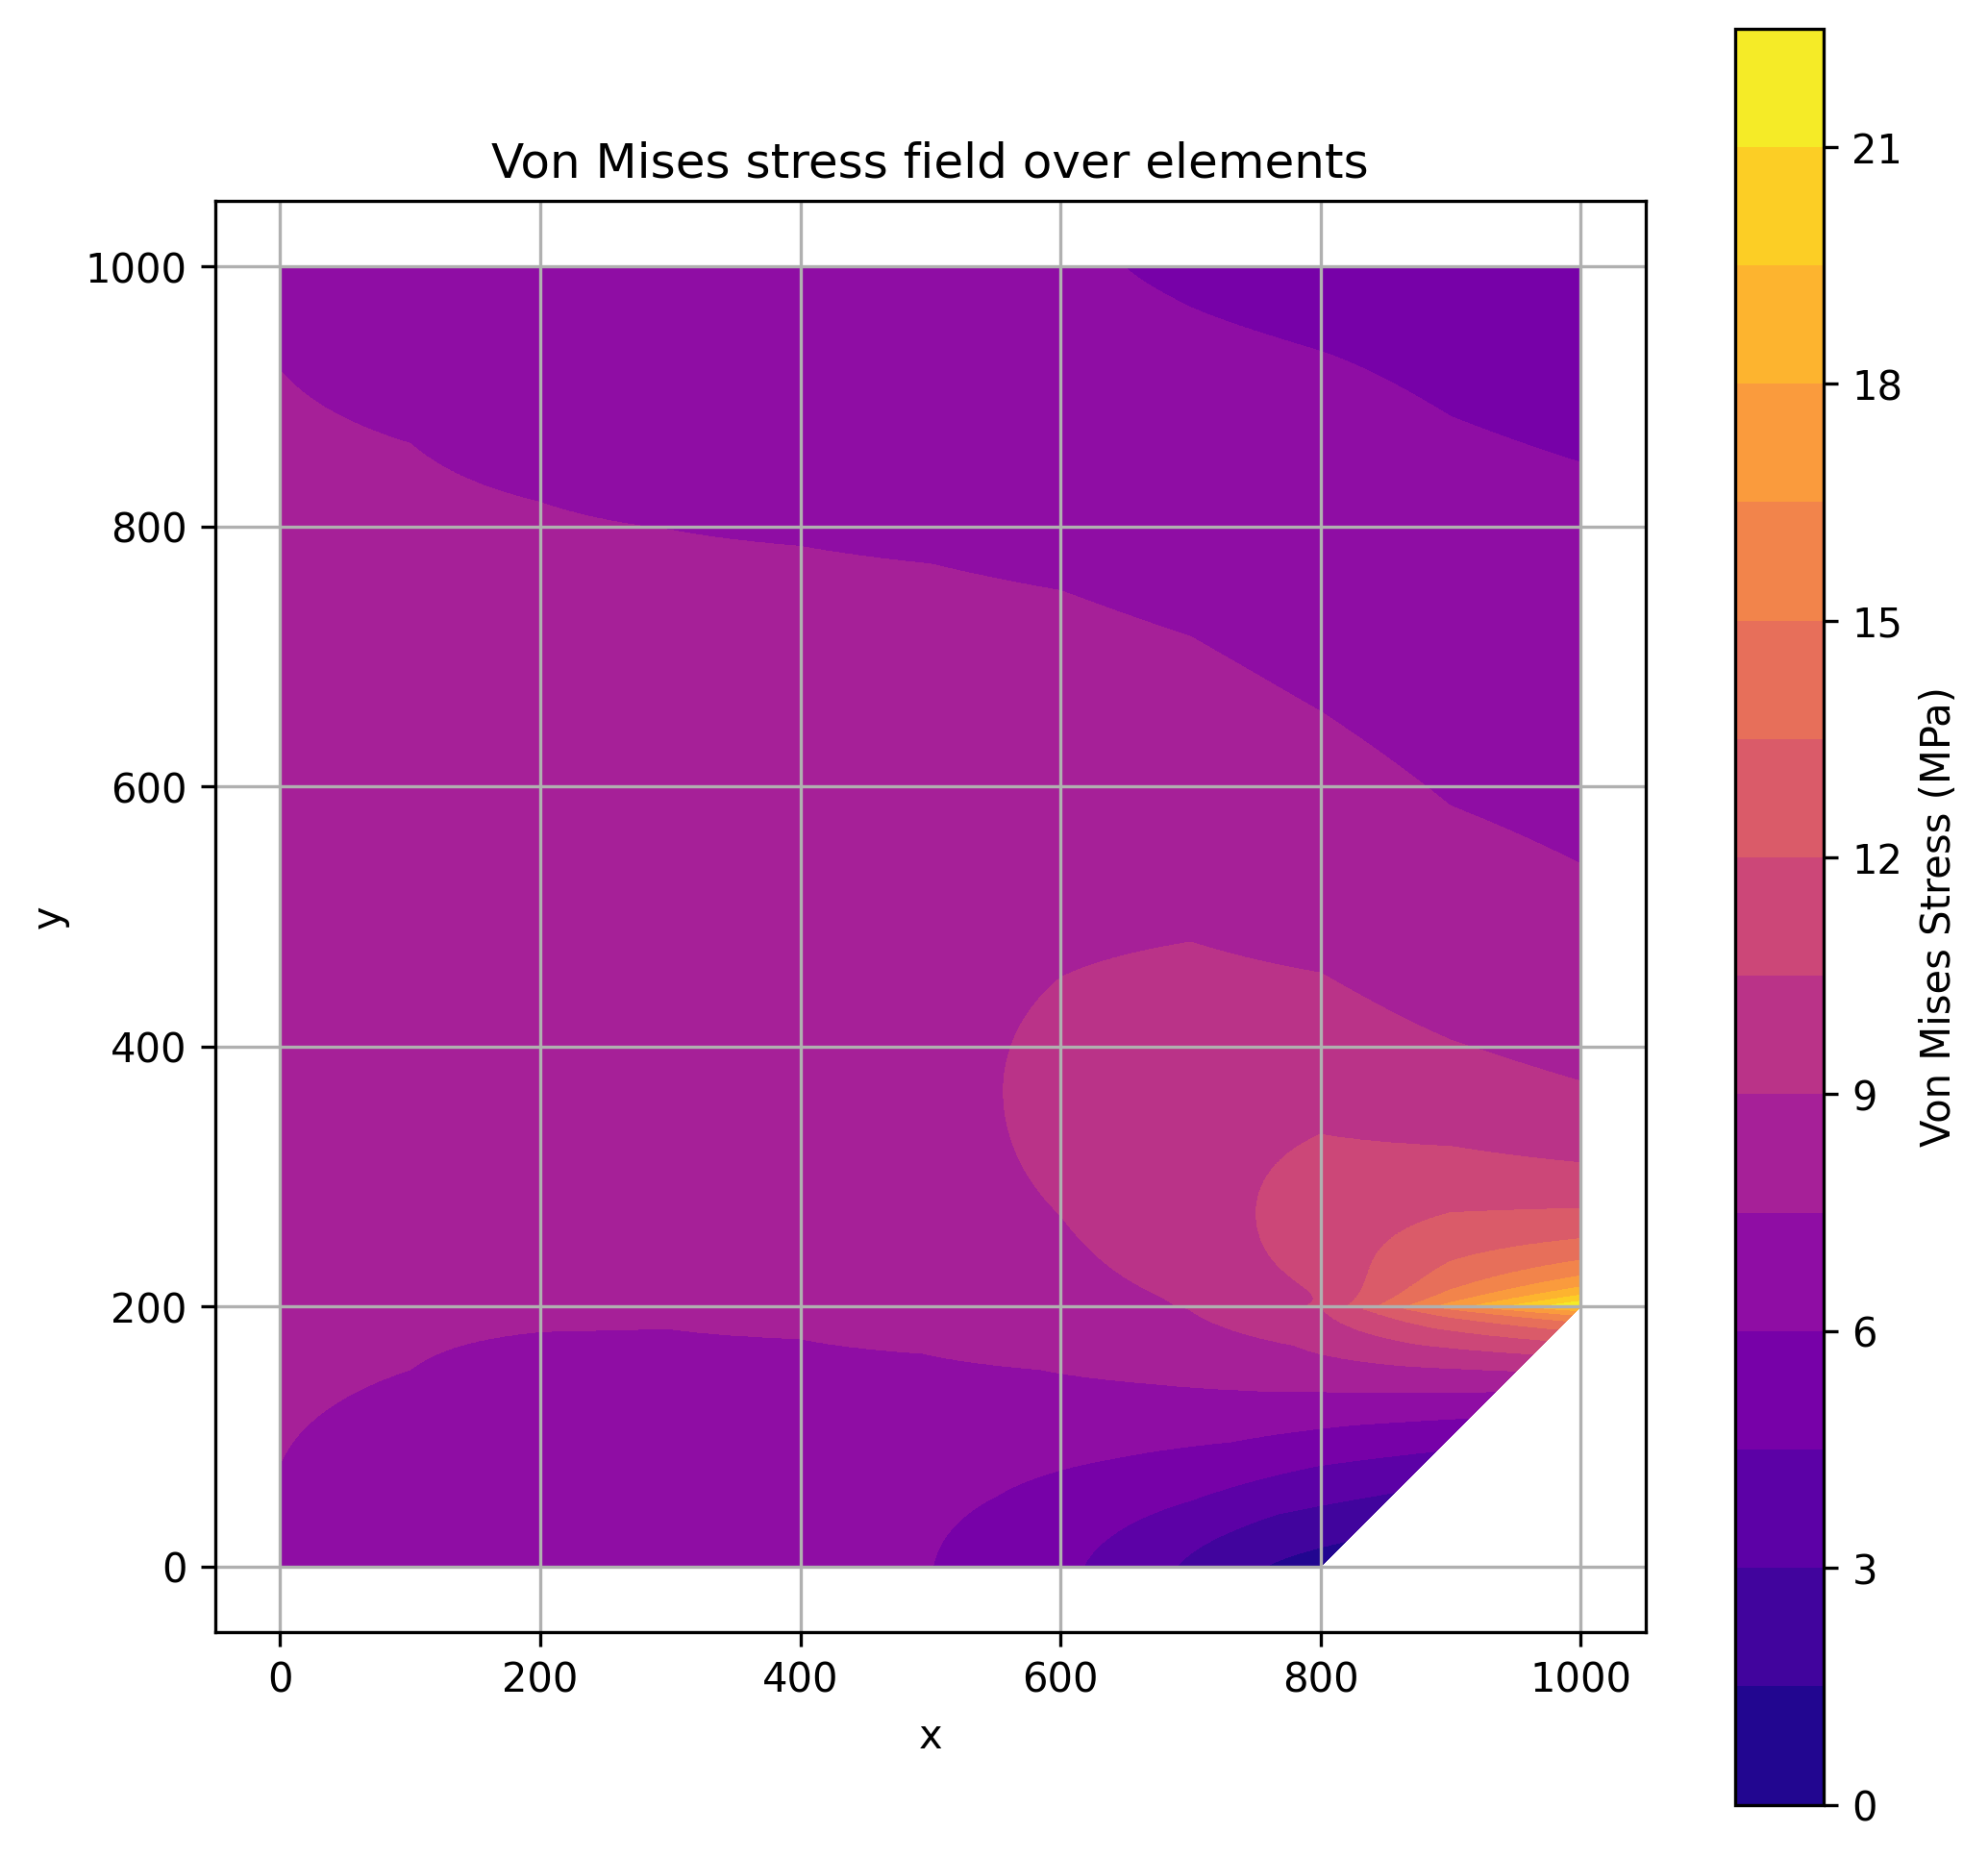
\includegraphics[width=\textwidth]{GRAFICOS/Quad9/1.25mm_global/resultados_von_mises.png}
    \caption{Local mesh refinement - $h=1.25mm$}
    \label{fig:img23}
  \end{subfigure}
\end{figure}

\subsection{Part c)}

In this section, an optimization of the strcutre was made. Moreover, it was modeled and simulated, reulting in a complete stress and behaviour analysis.

The main objective was to anulate the stress concentration sections, in order to reduce the maximum stress in the strcuture and compare it with the previous results.

